%\documentclass[10pt,oneside,reqno]{amsart}
\documentclass{article}

\usepackage{pgfplots}
\usepackage{tcolorbox}
\pgfplotsset{compat=1.15}
\usepackage{mathrsfs}
\usepackage{import}

\usepackage[mode=buildnew]{standalone}% requires -shell-escape

\usepackage[letterpaper,top=2cm,bottom=2cm,left=3cm,right=3cm,marginparwidth=1.75cm]{geometry}
%\setlength {\textwidth}{16.5truecm} 
%{\textheight}{22.0truecm} \calclayout

\usepackage{tikz}
\usepackage{tikz-3dplot}
\usepackage{pstricks-add}
\usetikzlibrary{arrows,shapes,positioning,shadows,trees}
\usetikzlibrary{arrows}
\usetikzlibrary{patterns}
\usetikzlibrary{calc}
\newtheorem{teo}{Théorème}
\newtheorem{lemma}[teo]{Lemme}
\newtheorem{prop}[teo]{Proposition}
\newtheorem{cor}[teo]{Corollaire}
\usepackage{tcolorbox}
\usepackage{wrapfig}
\usepackage{textcomp}
\usepackage{siunitx}
\def \be {\begin{equation*}}
\def \ee {\end{equation*}}
\def \dd  {{\rm d}}
\def \CFL {\beta_{CFL}}
\newcommand{\mail}[1]{{\href{mailto:#1}{#1}}}
\newcommand{\ftplink}[1]{{\href{ftp://#1}{#1}}}
\newcommand{\shrink}{\vspace{-1cm}}
\newcommand{\shrinkD}{\vspace{-0.5cm}}
\newcommand{\x}{\vec x}
\newcommand{\video}[2]{\nonfrench\href{#1}{#2}\endnonfrench\ }
\usepackage{cancel}
\usepackage{hyperref}
\hypersetup{
    colorlinks,
    citecolor=black,
    filecolor=black,
    linkcolor=black,
    urlcolor=black
}
\usetikzlibrary{decorations.pathmorphing}
\newcommand{\notimplies}{%
    \mathrel{{\ooalign{\hidewidth$\not\phantom{=}$\hidewidth\cr$\implies$}}}}
\newcommand{\Ressort}[4][]{
\node [minimum size=#2,#1] (ressort) at (#4) {};
\pgfmathparse{#2/#3}\let\pas\pgfmathresult
\draw [decorate,decoration={zigzag,segment length=\pas,amplitude=0.3cm}]
(ressort.east) -- (ressort.west);
}
\newtheorem{Exercice}{Exercice}[section]
\newtheorem{Corrige}{Corrigé}[section]
\newtheorem{Methode}{Methode}[section]



\DeclareMathAlphabet\mathzapf{T1}{pzc}{mb}{it}
\usepackage{wasysym}
\usepackage{latexsym}
\usepackage{float}
\usepackage{amssymb}
\usepackage{mathrsfs}
\usepackage{bm}
\usepackage{graphicx}
\usepackage{wrapfig}
\usepackage{fancybox}
\bibliographystyle{amsplain}
\usepackage{systeme}
\usepackage{pdfpages}
\usepackage{amsmath}

\usepackage{yfonts}
\usepackage[french]{babel}

\newtheorem{lemme}{Lemme}[subsection]
\newtheorem{assertion}{Assertion}[subsection]


\newtheorem{proposition}{Proposition}[section]
\newtheorem{corollaire}{Corollaire}[section]
\newtheorem{introduction}{Introduction}[section]
%\theoremstyle{definition}
\newtheorem{definition}{Définition}[section]
\newtheorem{savoirf}{Savoir-faire}[section]
\newtheorem{rem}{Remarque}[section]
\usepackage{subfigure}
\usepackage{titlesec}
\usepackage[titles,subfigure]{tocloft}
\usepackage{titletoc}
\setlength{\cftbeforesecskip}{3pt plus.2pt}
\renewcommand{\cftsecfont}{\bfseries}
\renewcommand{\cftsecpagefont}{\normalfont}
\renewcommand{\cftsecleader}{\normalfont\cftdotfill{\cftsecdotsep}}

\renewcommand{\cftsecdotsep}{\cftdotsep}
\cftpagenumbersoff{subsubsection}
%\cftpagenumbersoff{subsection}

\usepackage[T2A]{fontenc}


\title{Physique}
\author{\href{https://students-4-students.github.io}{\textcolor{black}{\underline{STUDENTS FOR STUDENTS}}}}
\date{Première édition - Septembre 2021}
\begin{document}

\maketitle
\vspace{6\baselineskip}
\begin{center}
   
\includegraphics[scale=1]{Images/ic_launcher.png} 
\end{center}


\pagenumbering{gobble}
\newpage $ $
\newpage
\nonumber
\newpage
\section*{Avant-propos}
%Insert foreword par Elias here: D'ailleurs Elias je te laisse rédiger, juste oublie pas de dire que cette brochure (je crois qu'on fait comme ça finalement, pour gagner du temps) est faite pour aider les enseignants-intervenants à approfondir, et pour aider les élèves à emporter pour l'année. C'est une \textbf{borne supérieure de difficulté}. Que les gens s'inquiètent pas en lisant ça et croyant qu'on va exploser les cerveaux des BA1 en une demi-journée alors que nos objectifs sont avant tout la concurrence avec les prépas, donner des bases de contact social et enfin seulement donner des bases académiques.

\subsection*{Mot du chef d'équipe, Elias Myers}

Ah la physique... Pas tout le monde la comprend, et encore moins de gens l'apprécient. C'est un peu la matière la moins aimée du premier semestre. En effet, c'est une matière complexe et qui sera probablement de peu d'intérêt pratique pour la suite de vos études en IC. 

Ce document a donc comme but de répondre à ces deux problèmes. D'abord, fournir une base et des rappels solides pour commencer à étudier la mécanique. Dedans, vous trouverez les notions qu'on aurait aimé savoir ou consolider avant de commencer le premier semestre. Ensuite, il s'agit d'essayer de trouver une certaine élégance dans cette matière, afin de montrer tout l'intérêt que ce cours peut avoir.

Pour cela, ce document est divisé en deux parties: d'abord un rappel de certaines notions de mathématiques, vues au lycée par certains, qui seront utiles en tout temps en physique. Ensuite, une introduction aux premiers sujets que vous aborderez pendant le semestre. C'est tout à fait normal si vous ne comprenez pas tout ce qui est écrit lorsque vous lisez ce document avant d'avoir commencé vos cours. Malgré nos meilleurs efforts, il y a certaines notions très complexes pour lesquelles plusieurs semaines de cours seront nécessaires pour les appréhender. Par ailleurs, le cours qui sera donné dans la matinée dans le cadre de S4S est une version simplifiée de ce document. 

J'en profite également pour formuler un petit avertissement. Ce cours de mécanique correspond à celui des IC, et donc celui de la majorité des sections de l'EPFL. En revanche, si vous êtes en architecture, ce cours va probablement trop loin par rapport à ce qui vous sera demandé. A l'inverse, si vous êtes en physique, ce cours risque d'être insuffisant comme préparation, car vous avez un cours de physique avancée. Je pense qu'il peut quand même être intéressant pour les physiciens de lire ce document, mais sachez qu'il n'est pas conçu pour vous préparer à ce qui vous attend. 

Je m'excuse aussi d'avance à tous ceux qui apprécient la rigueur mathématique, car vous risquez de faire 2-3 AVCs en lisant cette brochure. Vous verrez qu'en physique, beaucoup de raccourcis illégaux sont utilisés.

%Dans ce document nous utilisons de manière intervertible les notations $\vec{e}$ et $\mathbf{e}$

%Rajouter les inspirations ici aussi
\newpage
\tableofcontents
\newpage
\pagenumbering{arabic}

%\section{Introduction}
Avant toute chose, rappelons ce qu'est la mécanique. La mécanique est une branche de la physique qui consiste en l'étude du mouvement. Ce mouvement se caractérise de plusieurs manières, par son accélération, sa vitesse, sa position etc...  Le cours de BA1 correspondra à de la mécanique dite 'classique' qui étudie les mouvements d'objets macroscopiques, que ce soit les grains de poussière ou les comètes. Pour des objets très petits, comme les électrons, on ferait plutôt appel à la mécanique quantique, et pour des objets super rapides, la mécanique relativiste (voire même la mécanique quantique relativiste pour des petits objets rapides). Mais si vous voulez prédire le meilleur angle pour frapper une balle au baseball et faire un homerun, la mécanique classique est faite pour vous ! Néanmoins, avant d'être une branche de la physique, la mécanique était une branche des mathématiques. Avant de rentrer dans le vif du sujet, il est donc nécessaire de rappeler ou introduire certaines notions mathématiques.

\section{Mathématiques I}

\subsection{Dérivées et intégrales}
La grande majorité d'entre vous a déjà vu les dérivées et intégrales, mais une petite piqûre de rappel après les vacances ne fait pas de mal. Les techniques de dérivation et d'intégration ne seront pas présentées ici, car elles font plus partie du cursus d'analyse, et si vous n'êtes pas à l'aise avec la dérivation et l'intégration des fonctions de base, nous vous invitons fortement à vous renseigner de votre côté.

\subsubsection{Dérivées}
En physique, on utilise les dérivées pour représenter la variation infinitésimale d'une fonction par rapport à l'une de ses variables. Le plus souvent, on évalue la variation d'une fonction par rapport au temps, auquel cas il s'agit d'une dérivée temporelle. 


\begin{figure}[h]
    \centering
    \begin{center}
    
\definecolor{rvwvcq}{rgb}{0.08235294117647059,0.396078431372549,0.7529411764705882}
\begin{tikzpicture}[line cap=round,line join=round,>=triangle 45,x=2.077922077922078cm,y=2.6086956521739126cm]
\begin{axis}[
x=2.077922077922078cm,y=2.6086956521739126cm,
axis lines=middle,
ymajorgrids=true,
xmajorgrids=true,
xmin=-0.05,
xmax=3.8,
ymin=-0.05,
ymax=1.1,
xtick={-0.0,0.5,...,3.5},
ytick={-0.0,0.5,1.0},]
\clip(-0.05,-0.05) rectangle (3.8,1.1);
\draw[line width=4.pt] (-0.086090907575987,1.6578211468632087) -- (0.49556511308165885,1.6578211468632087);
\draw[line width=4.pt] (-0.35074439697521587,1.7567026703750082) -- (0.23091162368243,1.7567026703750082);
\begin{scriptsize}
\draw [fill=black] (0.08840589862130677,1.6578211468632087) circle (2.5pt);
\draw[color=black] (0.10003901903445966,1.726165729290482) node {$t = 3$};
\draw [fill=black] (-0.187880711191075,1.7567026703750082) circle (2.5pt);
\draw[color=black] (-0.14134822953846338,1.8250472528022814) node {$v0 = -5.8$};
\draw [fill=rvwvcq] (3.,0.5921521997621881) circle (2.5pt);
\draw[color=rvwvcq] (3.1,0.7) node {$P$};
\draw[color=black] (3.55,0.1) node {$x(t)$};
\draw[color=black] (0.2,1.025) node {$y(t)$};
\draw [fill=rvwvcq] (0.1,0.09732461355529132) circle (2.5pt);
\draw [fill=rvwvcq] (0.3,0.2759215219976218) circle (2.5pt);
\draw [fill=rvwvcq] (0.4,0.3571938168846611) circle (2.5pt);
\draw [fill=rvwvcq] (0.5,0.43311533888228293) circle (2.5pt);
\draw [fill=rvwvcq] (0.6,0.5036860879904874) circle (2.5pt);
\draw [fill=rvwvcq] (0.7,0.5689060642092746) circle (2.5pt);
\draw [fill=rvwvcq] (1.,0.7324613555291319) circle (2.5pt);
\draw [fill=rvwvcq] (1.1,0.7762782401902496) circle (2.5pt);
\draw [fill=rvwvcq] (1.4,0.8756242568370985) circle (2.5pt);
\draw [fill=rvwvcq] (1.6,0.9151010701545779) circle (2.5pt);
\draw [fill=rvwvcq] (1.7,0.9268133174791915) circle (2.5pt);
\draw [fill=rvwvcq] (1.9,0.9341854934601663) circle (2.5pt);
\draw [fill=rvwvcq] (2.3,0.8847205707491081) circle (2.5pt);
\draw [fill=rvwvcq] (2.4,0.8589774078478003) circle (2.5pt);
\draw [fill=rvwvcq] (2.5,0.8278834720570747) circle (2.5pt);
\draw [fill=rvwvcq] (2.8,0.7024970273483948) circle (2.5pt);
\draw [fill=rvwvcq] (2.9,0.65) circle (2.5pt);
\draw [fill=rvwvcq] (3.,0.5921521997621881) circle (2.5pt);
\end{scriptsize}
\end{axis}
\end{tikzpicture}
\end{center}

    \caption{La position d'un projectile est une fonction du temps}
    \label{fig:xt}
\end{figure}
Je m'explique avec un exemple simple. Considérons une fonction position $x(t)$, qui mesure la position d'un point matériel $P$ le long d'un axe. Au cours du temps, cette position varie. On peut donc mesurer cette variation pendant un certain intervalle de temps, puis diviser par la durée de cet intervalle, afin d'obtenir le rapport entre la variation de position et le temps écoulé (c'est d'ailleurs le principe de la vitesse moyenne, que vous avez déjà vu au gymnase). Si l'on fait tendre cet intervalle de temps vers $0$, on obtient la vitesse instantanée. En physique, vous utilisez quasiment toujours la vitesse instantanée, qui sera simplement nommée vitesse. La vitesse est donc simplement la dérivée temporelle de la position. On appelle cela une dérivée temporelle car la vitesse mesure la \textit{variation de la position \textit{en fonction de $t$}}. On peut faire un raisonnement similaire et observer que l'accélération est la dérivée temporelle de la vitesse. \\

\begin{tcolorbox}[title=Notation des dérivées temporelles, enlarge top by=1mm, enlarge bottom by=1mm]
\[
    \lim_{\Delta t \to 0} \frac{x(t + \Delta t) - x(t)}{\Delta t} = \frac{dx(t)}{dt} = \dot{x}(t) = x'(t)
\]
\end{tcolorbox}

Pour rappel, en physique $\vec{r}(t)$ représente la position, $\vec{v}(t)$ la vitesse et $\vec{a}(t)$ l'accélération. Grâce aux observations que nous venons de faire, on peut conclure : 
\[\boxed{ \vec{a}(t) = \dot{\vec{v}}(t) = \ddot{\vec{r}}(t).}\]

Les plus attentifs auront remarqué une petite subtilité dans ce qui précède. En effet $\vec{r}(t)$, $\vec{v}(t)$ et $\vec{a}(t)$ ne sont pas des fonctions scalaires mais des fonctions vectorielles ! Cependant, dans les cas simples, on peut simplement \textit{dériver un vecteur en dérivant chacune de ses composantes} (Vous verrez un exemple de cas complexe dans le chapitre de mécanique II). De manière alternative, on peut utiliser la définition de la dérivée avec une fonction vectorielle:  \[ \boxed{ \lim_{\Delta t \to 0} \frac{\vec{r}(t + \Delta t) - \vec{r}(t)}{\Delta t}} \]

\indent Cette formule peut être mieux comprise grâce à la Figure 2. On a un point matériel qui se déplace sur une trajectoire $\Gamma$. On mesure la position $\vec{r}_1$ à un instant $t_1$, et plus tard la position $\vec{r}_2$ au temps $t_2$. On peut ensuite calculer le déplacement $\vec{d} = \vec{r}_2 - \vec{r}_1$ entre ces deux positions. Comme ce déplacement à eu lieu durant un certain intervalle de temps, on divise ensuite par la durée de cet intervalle. Vous remarquez donc qu'on fait bien exactement la même chose que dans les dérivées des fonctions que vous avez eu l'habitude de voir.

\begin{figure}
    \centering

\definecolor{qqwuqq}{rgb}{0,0.39215686274509803,0}
\definecolor{qqqqff}{rgb}{0,0,1}
\definecolor{ccqqqq}{rgb}{0.8,0,0}
\begin{tikzpicture}[line cap=round,line join=round,>=triangle 45,x=1cm,y=1cm]
\begin{axis}[
x=1cm,y=1cm,
axis lines=middle,
xmin=-1,
xmax=8.385055628710091,
ymin=-1.4004451090161362,
ymax=5.386008244213317,
xtick={-3,-2,...,8},
ytick={-1,-0,...,5},]
\clip(-1,-1.4004451090161362) rectangle (8.385055628710091,5.386008244213317);
\draw [shift={(1.9833804,-0.1)},line width=1.2pt]  plot[domain=1.1705556697609223:2.527573616581852,variable=\t]({1*2.5368001936194266*cos(\t r)+0*2.5368001936194266*sin(\t r)},{0*2.5368001936194266*cos(\t r)+1*2.5368001936194266*sin(\t r)});
\draw [->,line width=0.8pt,color=ccqqqq] (0,0) -- (1.8083053066921226,3.5480972786760643);
\draw [->,line width=0.8pt,color=qqqqff] (0,0) -- (3.493475720586349,3.8426391465182914);
\draw [->,line width=0.8pt,color=qqwuqq] (1.8083053066921226,3.5480972786760643) -- (3.493475720586349,3.8426391465182914);
\begin{scriptsize}
\draw[color=black] (2.437137873052433,3.9683145856067447) node {$\Gamma$};
\draw[color=ccqqqq] (1.2940596701619935,2.0567376724981345) node {$\vec{r}_1$};
\draw[color=qqqqff] (2.0899578644674388,1.9359316965767727) node {$\vec{r}_2$};
\draw[color=qqwuqq] (2.350837615096068,3.413002891720386) node {$\vec{d}$};
\end{scriptsize}
\end{axis}
\end{tikzpicture}
    \caption{Vecteur déplacement et intuition derrière la dérivée vectorielle}
    \label{fig:deriveeVect}
\end{figure}

Vous verrez aussi au cours du semestre certaines formules qui peuvent aider à dériver un vecteur dans certaines situations (cf les lois de Poisson).

\subsubsection{Intégrales}
Rechercher une primitive est l'opération inverse du calcul de la dérivée. Ainsi, soit $F(x)$ une fonction telle que $F'(x) = f(x)$, alors on dit que $F(x)$ est une primitive de $f(x$). Pour rappel, les primitives sont calculées à une constante près. En effet, soit $F(x)$ une primitive de $f(x)$, alors $F(x) + C$ est aussi une primitive de $f(x)$, pour tout $C \in \mathbb{R} $. Ceci sera d'une importance capitale en mécanique, lorsque vous recherchez les équations horaires des objets étudiés. \\

On peut donc constater que la primitive de l'accélération (à une constante près) est la vitesse, et que la primitive de la vitesse (à une constante près) est la position. \\

\noindent \textbf{Théorème Fondamental de l'analyse}\\
L'intégrale d'une fonction $f$ entre deux points $a$ et $b$ est égale à l'aire entre le graphe de cette fonction et l'axe des abscisses. Contrairement à la primitive, il s'agit donc d'un nombre, et non d'une fonction. Elle est notée ainsi:
\[\int_{a}^{b}f(x) \,dx\]

\noindent En analyse, vous verrez deux théorèmes fondamentaux de l'analyse. On présentera ici le second, qui permet de calculer l'aire sous la courbe, et qui est beaucoup plus utile en physique:
\begin{tcolorbox}[title=Théorème fondamental de l'analyse, enlarge top by=1mm, enlarge bottom by=1mm]
Soit $f(x)$ une fonction continue sur un intervalle $[a;b]$. Si $F(x)$ est une primitive de $f(x)$ sur cet intervalle, alors:
\[\int_{a}^{b}f(x) \,dx = F(b) - F(a)\]
\end{tcolorbox}


\noindent \textbf{Confusion entre fonction et variable}


Une confusion fréquente au début est due au fait qu'on ne se rappelle pas toujours de ce qu'on dérive, et par rapport à quoi. Prenons un exemple tout simple. On souhaite dériver $\sin{(\theta)}$ par rapport au temps. Ici $\theta$ représente un angle utilisé pour décrire la position du point matériel.  L'erreur fréquente serait de dire que sa dérivée est simplement $\cos{\theta}$. Pourquoi est-ce faux ? Tout simplement parce que $\theta$ est une fonction du temps $t$. On note en effet $\theta$ comme raccourci à la fonction $\theta (t)$. La dérivée correcte est donc \[ \frac{d}{dt} (\sin{\theta}) = \cos{(\theta)} \dot{\theta}.\]
Pour ceux qui ont du mal à comprendre pourquoi, rappelez-vous de la formule de dérivation d'une composition: 
\[ (f(g(x))' = f'(g(x)) g'(x) \]
Si vous remplacez la fonction $f$ par $\sin$ et $g$ par $\theta$, ainsi que la variable $x$ par $t$, vous voyez qu'on obtient bien effectivement $\cos{(\theta)} \dot{\theta}.$


\subsection{Produit scalaire et produit vectoriel}
Il s'agit probablement aussi de notions déjà vues au gymnase pour la plupart d'entre vous, mais il est important qu'elles soient absolument sans secret pour vous. 
\subsubsection{Décomposition d'un vecteur par rapport à un autre} 
Avant d'étudier le produit scalaire et le produit vectoriel, il est important de faire l'observation suivante:
pour toute paire de vecteurs $(\vec{a}, \vec{b})$, on peut décomposer le vecteur $\vec{a} $ en deux vecteurs, un vecteur $ \vec{a}_\parallel $ parallèle au vecteur $\vec{b}$  et un vecteur $\vec{a}_\bot $,  perpendiculaire à $\vec{b}$, tels que $ \vec{a} = \vec{a}_\parallel\ + \vec{a}_\bot $. Vous verrez plus tard que cette décomposition est indispensable dans tout problème de mécanique.

\begin{figure}[ht]
\begin{center}
\definecolor{ffzzqq}{rgb}{1,0.6,0}
\definecolor{qqqqff}{rgb}{0,0,1}
\definecolor{ffqqqq}{rgb}{1,0,0}
\definecolor{uuuuuu}{rgb}{0.26666666666666666,0.26666666666666666,0.26666666666666666}
\begin{tikzpicture}[line cap=round,line join=round,>=triangle 45,x=1cm,y=1cm]
\begin{axis}[
x=1cm,y=1cm,
axis lines=middle,
xmin=-1,
xmax=8.455900440737476,
ymin=-0.3726406540327187,
ymax=4.998307713421168,
xtick={-1,0,...,8},
ytick={-2,-1,...,4},]
\clip(-1.1821895493954007,-2.3726406540327187) rectangle (8.455900440737476,4.998307713421168);
\draw [->,line width=1.2pt,color=ffqqqq] (0,0) -- (3.35571,3.23601);
\draw [->,line width=1.2pt,color=qqqqff] (0,0) -- (6.984054440553234,2.1760419327496505);
\draw [->,line width=1.2pt,color=ffzzqq] (3.96723,1.19761) -- (3.35571,3.23601);
\draw [->,line width=1.2pt,color=ffzzqq] (0,0) -- (3.96723,1.19761);
\begin{scriptsize}
\draw [fill=uuuuuu] (0,0) circle (2pt);
\draw[color=ffqqqq] (1.5873326976668879,1.8837856542120805) node {$\vec{a}$};
\draw[color=qqqqff] (5.0000000000000001,1.2690240297390751) node {$\vec{b}$};
\draw[color=ffzzqq] (3.8847125080196666,2.3642615286178104) node {$a_\bot$};
\draw[color=ffzzqq] (2.0378086973080833,0.8590242802100065) node {$a_\parallel$};
\end{scriptsize}
\end{axis}
\end{tikzpicture}
\end{center}
\caption{Décomposition du vecteur $\vec{a}$ par rapport au vecteur $\vec{b}$}
    \label{fig:polar}
\end{figure}

%PRODUIT SCALAIRE
\subsubsection{Produit scalaire}
Le produit scalaire est une opération algébrique qui retourne un scalaire (un nombre) pour chaque paire de vecteurs. Ce scalaire donne une indication du point auquel deux vecteurs sont parallèles.

\begin{tcolorbox}[title=Calcul de produit scalaire, enlarge top by=1mm, enlarge bottom by=1mm]
 Soient deux vecteurs dans l'espace $\vec{a} = (a_1, a_2, a_3) $ et $\vec{b} = (b_1, b_2, b_3)$ et $\alpha$ l'angle entre eux. Alors leur produit scalaire vaut : \[ \vec{a} \cdot \vec{b} = a_1 b_1 + a_2 b_2 + a_3 c_3 = \lVert \vec{a} \rVert \lVert \vec{b} \rVert \cos(\alpha)\]
\end{tcolorbox}

La formule à utiliser pour le calcul du produit scalaire dépendra de comment les vecteurs $\vec{a}$ et $\vec{b}$ sont donnés. On utilise la première formule lorsque les coordonnées des vecteurs sont données, et la seconde lorsque l'on a les normes et l'angle des vecteurs. Vous pouvez d'ailleurs vous amuser à montrer que les deux formules sont équivalentes. 

À partir de ces formules, on peut facilement conclure certaines propriétés importantes du produit scalaire. Ces propriétés seront très souvent utilisées pour simplifier des calculs:

\begin{tcolorbox}[title = Propriétés du produit scalaire, enlarge top by=1mm, enlarge bottom by=1mm]
On note $\perp$ pour perpendiculaire, et $||$ pour parallèle.
\begin{align*}
    \vec{u} \perp \vec{v} &\iff \vec{u} \cdot \vec{v} = 0\\
\vec{u} \: || \: \vec{v} &\iff \vec{u} \cdot \vec{v} = \pm \lVert \vec{u} \rVert \lVert \vec{v} \rVert
\end{align*}
\textbf{Exercice :}

\begin{enumerate}
    \item Que peut-on dire de $\vec{a}$ et $\vec{b}$ si $\vec{a} \cdot \vec{b} < 0 $ ? 
    \item Que vaut $\vec{a} \cdot \vec{a}$ ?
    \item Montrer que $\vec{a} \cdot \vec{b} = \vec{b} \cdot \vec{a}$
\end{enumerate}
\end{tcolorbox}

\subsubsection{Produit vectoriel} Le produit vectoriel est, quant à lui, une opération algébrique qui associe un vecteur $\vec{c}$ à chaque paire de vecteurs $\vec{a}$ et $\vec{b}$. Ce vecteur donne une indication du point auquel deux vecteurs sont perpendiculaires. 
Le vecteur obtenu $\vec{c}$ est de norme $\lVert \vec{a} \rVert \lVert \vec{b} \rVert \sin{\alpha}$, et est perpendiculaire au plan généré par $\vec{a}$ et $\vec{b}$. Le sens du vecteur $\vec{c}$ est celui dans lequel le triplé de vecteurs $(\vec{a}, \vec{b}, \vec{c})$ satisfait la règle de la main droite.

\begin{figure}[ht]

\begin{center}
\begin{tikzpicture} %[scale=1.2, every node/.style={scale=1.2}]
   \draw[-,fill=white!95!red](0,0)--(3,0)--(4,1)--(1,1)--cycle;
\node at (2,0.5) {$\lVert \vec{a} \times \vec{b} \rVert$};
\draw[line width=1.2pt,-latex,blue](0,0)--(3,0)node[midway,below]{$\vec{a}$};
\draw[line width=1.2pt,-latex,red](0,0)--(1,1)node[midway,above]{$\vec{b}$};
\draw[line width=1.0pt,-latex,green](0,0)--(0,3)node[pos=0.7,right]{$\vec{c} = \vec{a} \times \vec{b}$};
\draw (0.6,0) arc [start angle=0,end angle=45,radius=0.6]
node[pos=0.7,right]{$\theta$};
\end{tikzpicture}
\end{center}

\caption{Illustration du produit vectoriel}
    \label{fig:produitvec}
\end{figure}

La règle de la main droite sert à savoir dans quel sens mettre le troisième vecteur. Typiquement, dans cet exemple, il faut savoir si $\vec{c}$ va vers le haut ou vers le bas. Suivez cette règle pour le savoir!

\noindent\begin{minipage}{0.85\textwidth}
\setlength{\parindent}{0.5cm}
 Faites le en même temps que vous lisez ces lignes. Prenez votre main \textbf{droite} et mettez la paume face à vous. Tendez le pouce et l'index et tendez le majeur vers vous. Vous devriez voir que chaque doigt est perpendiculaire par rapport à l'autre. Eh bien si votre premier axe est votre pouce, le deuxième votre index, alors le dernier est votre majeur. Cela vous renseigne sur le sens du dernier vecteur. 

Pour anecdote, cette règle de la main droite est tellement importante qu'elle est même illustrée sur les billets de banque suisses de 200 francs. 

D'ailleurs, rien ne vous empêche d'en prendre un à l'examen pour bien vous rappeler la règle de la main droite. Vous pouvez même le laisser dans votre copie pour de meilleurs résultats.


\end{minipage}
\begin{minipage}{0.15\textwidth}
\centering
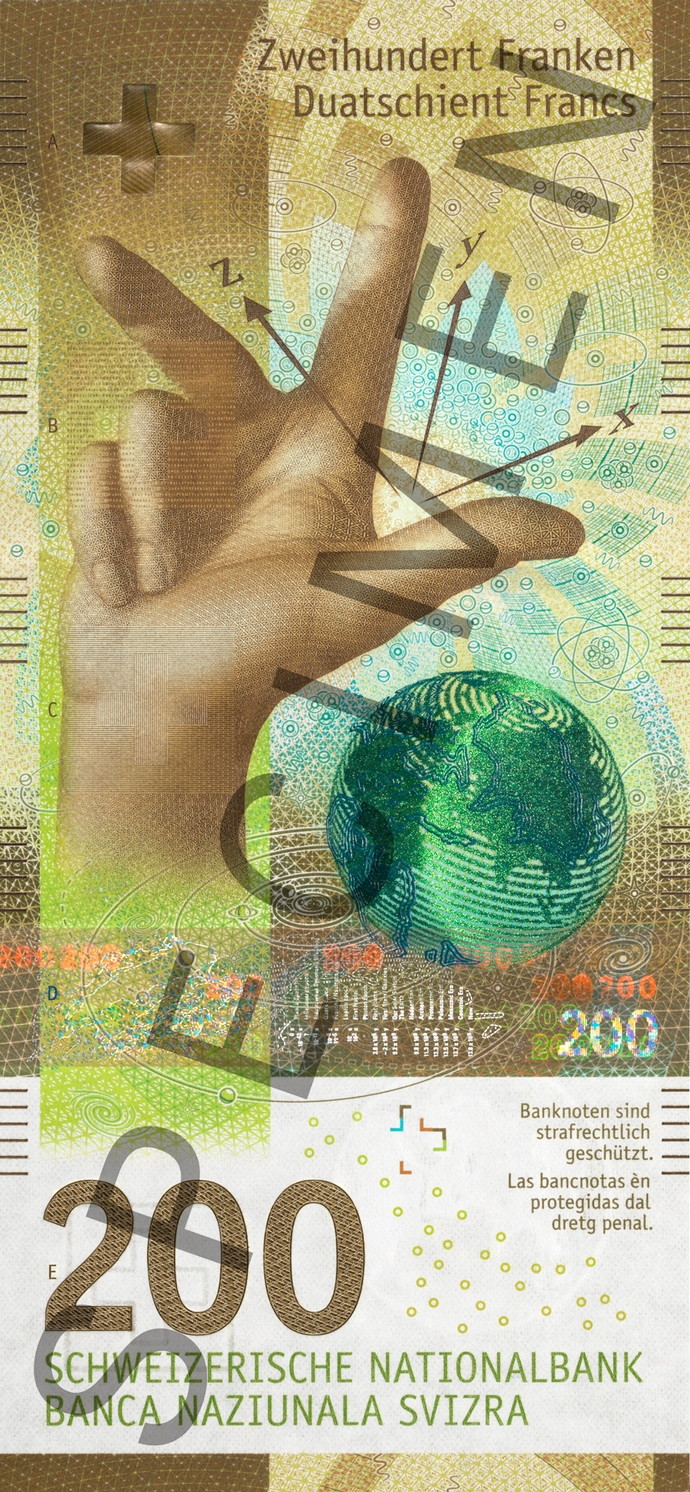
\includegraphics[width=0.85\textwidth]{Images/billet_200.jpg}
\end{minipage}




\begin{tcolorbox}[title = Calcul du produit vectoriel, enlarge top by=1mm, enlarge bottom by=1mm]
Soient $\Vec{a}=(a_1,a_2,a_3),\Vec{b}=(b_1,b_2,b_3)$ des vecteurs décrits selon la base canonique $(\mathbf{e}_1,\mathbf{e}_2,\mathbf{e}_3).$ Alors le calcul du produit vectoriel dans $\mathbb{R}^3$ peut se faire en calculant le déterminant de la matrice suivante :\begin{align*}
    \vec{a} \times \vec{b}& = \begin{vmatrix}\mathbf{e}_1 & \mathbf{e}_2 & \mathbf{e}_3\\
a_1 & a_2 & a_3\\
b_1 & b_2 & b_3\end{vmatrix}=\begin{pmatrix}
a_2 b_3 - a_3 b_2 \\
a_3 b_1 - a_1 b_3 \\
a_1 b_2 - a_2 b_1
\end{pmatrix}
\end{align*}
 
\end{tcolorbox}


\textbf{Exercice :} 
\begin{enumerate}
    \item Montrer que l'aire du parallélogramme généré par $\vec{a}$ et $\vec{b}$ vaut $\lVert \vec{a} \times \vec{b} \rVert$
    \item Montrer que le produit vectoriel est antisymétrique, c'est-à-dire que $\vec{a} \times \vec{b} = - \vec{b} \times \vec{a}$. Sauriez vous expliquer pourquoi ?
    \item Que vaut $\vec{a} \times \vec{a} ?$
    \item Soit $\Vec{a}=(3,2,1), \Vec{b}=(4,5,6)$. Arriveriez-vous à calculer $\vec{a} \times \vec{b},$ en utilisant la formule utilisant le déterminant donné ci-dessus ?
\end{enumerate}


\begin{tcolorbox}[title = Propriété du produit vectoriel, enlarge top by=1mm, enlarge bottom by=1mm]

Soit $\vec{u}$ parallèle à $\vec{v}$, alors $\vec{u} \times \vec{v} = \vec{0}$
\end{tcolorbox}

\subsection{Projections}

Dans vos exercices de méca, il sera quasiment  indispensable de décomposer vos forces, et donc de calculer leurs projections sur chaque axe de votre repère.
Savoir projeter vos forces est donc un skill ultra important en physique, il est nécessaire de le réaliser rapidement et sans faute. Sinon, tout le reste de votre raisonnement est faux. Beaucoup de personnes perdent du temps et des points à l'examen à cause de ça.


On peut bien évidemment apprendre par coeur comment projeter ses forces, mais le mieux reste de savoir d'où cela vient. 
Dans le schéma ci-dessous, on veut projeter le vecteur $\vec{r}$, de norme $r$ et d'orientation $\alpha$, sur le repère orthonormé constitué des vecteurs $\vec{e}_x$, $\vec{e}_y$ et de centre $O$. Le vecteur $\vec{r}$ est le même que $\overrightarrow{OA}$. Le point A est identifié par ses coordonnées qu'on note souvent \[A=(r_x; r_y)\]
 où $r_x$ est la projection du vecteur $\vec{r}$ sur l'axe $x$, et $r_y$ celle sur l'axe $y$. Mais on peut aussi dire que le vecteur \[\overrightarrow{OA}=\vec{r}=r_x \vec{e}_x+r_y \vec{e}_y\]
où $\vec{e}_x$ et $\vec{e}_y$ sont les vecteurs de la base. Ils ont comme norme 1 dans ce cas-là car le repère est orthonormé. Mais ces vecteurs définissent en quelque sorte une échelle. \\
Il existe plusieurs manières de trouver $r_x$ et $r_y$, et personnellement j'aime bien utiliser Thalès.
\begin{figure}[H]

\definecolor{ffqqqq}{rgb}{1,0,0}

\begin{center}
    

\begin{tikzpicture}[line cap=round,line join=round,>=triangle 45,x=1cm,y=1cm]

\begin{axis}[
x=3cm,y=3cm,
axis lines=middle,
xmin=-0.5142915773407036,
xmax=2.181198209028875,
ymin=-0.39259802589438797,
ymax=1.6688390493632528,
xtick={-0.0},
ytick={-0.0},]
\clip(-0.5142915773407036,-0.39259802589438797) rectangle (2.181198209028875,1.6688390493632528);
\draw [->,line width=1.2pt] (0,0) -- (1,0);
\draw [->,line width=1.2pt] (0,0) -- (0,1);
\draw [->,line width=2pt,color=ffqqqq] (0,0) -- (1.5,1.2);
\draw [line width=0.4pt] (0,0) circle (3cm);
\draw [line width=0.8pt] (1.5,1.2)-- (1.5,0);
\draw [line width=0.8pt] (1.5,1.2)-- (0,1.185711555344861);
\draw [line width=0.8pt] (0.7804878048780488,0.624390243902439)-- (0.78,0);
\draw [line width=0.8pt] (0,0.62)-- (0.7804878048780488,0.624390243902439);
\draw (0.6457929204990373,-0.04841070846721544) node[anchor=north west] {$\cos{\alpha}$};
\draw (-0.327101962415107,0.7018961917741242) node[anchor=north west] {$\sin{\alpha}$};
\begin{scriptsize}
\draw[color=black] (0.5179584885758282,0.0822658755554778) node {$\vec{e}_x$};
\draw[color=black] (0.07624777596115196,0.5370396447455734) node {$\vec{e}_y$};
\draw[color=ffqqqq] (0.8671469381737054,0.7698319444774911) node {$\vec{r}$};
\draw[color=black] (1.65,0.6289313420081725) node {$r_y$};
\draw[color=black] (0.7721921843356863,1.2629840531201064) node {$r_x$};
\draw[color=black] (2.1,0.05) node {$x$};
\draw[color=black] (0.05,1.56) node {$y$};

\end{scriptsize}
\end{axis}
\end{tikzpicture}

\end{center}

\caption{Projection du vecteur $\Vec{r}$ sur un repère orthonormé}
    \label{fig:proj}
\end{figure}


 \noindent Par Thalès, on a les relations suivantes:

\[ \frac{1}{r} = \frac{\cos{\alpha}}{r_x} = \frac{\sin{\alpha}}{r_y}\] En remaniant ces équations, on trouve facilement : 


\[\boxed{ r_x = r \cos{\alpha}\qquad r_y = r \sin{\alpha}} \]

\vspace{0.3cm}


\noindent Pour trouver $r_x$ et $r_y$, on peut aussi utiliser le produit scalaire. Si dans notre base on a $\mathbf{e_x}$ et $\mathbf{e_y}$ des vecteurs unitaires, alors on peut observer que:
\[r_x=\vec{r} \cdot \vec{e}_x=\lVert \vec{r}\rVert \lVert \vec{e}_x\rVert \cos{(\alpha)}=r\cos{(\alpha)}\]
car le vecteur $\vec{e}_x$ est de norme 1. On peut faire un raisonnement similaire avec $r_y$, en se rappelant que $\cos{(\frac{\pi}{2}-\alpha)} = \sin{\alpha}$. Nous verrons à travers les exemples dans la partie mécanique l'usage de ce produit scalaire. 



\noindent\textbf{Exercice}: Retrouver les mêmes formules en utilisant les propriétés de $\sin$ et $\cos$ dans un triangle rectangle (sohcahtoa)

\newpage

\section{Mathématiques II}

%DEVELOPPEMENT LIMITES
\subsection{Approximation et développements limités}
Comme vous le verrez, en physique, on approxime très souvent les résultats afin d'obtenir des formules plus sympathiques à utiliser.
Pour cela, nous utilisons les développements limités (aussi appelés développements de Taylor, vus à la fin du semestre en analyse), qui permettent d'approximer une fonction à l'aide d'un polynôme, car un polynôme est quand même beaucoup plus simple à étudier qu'une fonction complexe. 

A quoi cela peut-il bien nous servir en physique ? Eh bien, on s'en sert typiquement pour approximer les fonctions trigonométriques, en particulier cosinus et sinus autour de 0. En regardant les graphes de ces fonctions (\autoref{fig:dl}), vous verrez assez facilement par quoi on peut les approximer. Pour le cosinus, vous pouvez facilement voir qu'autour de 0, $\cos{x}$ vaut environ 1.  Pour le sinus, on voit que la plus simple approximation est simplement $x$. 

Vous pouvez vous demander pourquoi on approxime cosinus par une constante et le sinus par une fonction affine. La réponse complète se trouve dans le prochain paragraphe, mais elle utilise des notions d'analyse que vous verrez en fin de semestre, il n'est donc pas attendu que vous les connaissiez. Je peux cependant essayer de donner une explication visuelle. Si on se borne à approximer le cosinus avec une droite, il n'est tout simplement pas possible de faire une meilleure approximation que celle de la fonction constante 1. En effet, dès que vous rajoutez une pente à cette droite, elle va certes être une meilleure approximation d'un côté de l'axe $y$, mais une moins bonne de l'autre côté. L'approximation de $\cos(x)$ par 1 est toujours la meilleure approximation par une droite. 

\begin{figure}[ht]

\begin{center}
\definecolor{ccqqqq}{rgb}{0.8,0,0}
\definecolor{qqqqff}{rgb}{0,0,1}
\begin{tikzpicture}[line cap=round,line join=round,>=triangle 45,x=1cm,y=1cm]
\begin{axis}[
x=1cm,y=1cm,
axis lines=middle,
xmin=-2.5400689538405253,
xmax=2.536515566558789,
ymin=-2.111629827594053,
ymax=2.178011872488389,
xtick={-2,-1,...,2},
ytick={-2,-1,...,2},]
\clip(-2.8400689538405253,-2.111629827594053) rectangle (3.136515566558789,2.478011872488389);
\draw[line width=0.8pt,color=qqqqff,smooth,samples=100,domain=-2.8400689538405253:3.136515566558789] plot(\x,{cos(((\x))*180/pi)});
\draw [line width=0.8pt,color=ccqqqq,domain=-2.8400689538405253:3.136515566558789] plot(\x,{(--1-0*\x)/1});
\end{axis}
\end{tikzpicture}
%
\definecolor{ccqqqq}{rgb}{0.8,0,0}
\definecolor{qqqqff}{rgb}{0,0,1}
\begin{tikzpicture}[line cap=round,line join=round,>=triangle 45,x=1cm,y=1cm]
\begin{axis}[
x=1cm,y=1cm,
axis lines=middle,
xmin=-2.5400689538405253,
xmax=2.536515566558789,
ymin=-2.111629827594053,
ymax=2.178011872488389,
xtick={-2,-1,...,2},
ytick={-2,-1,...,2},]
\clip(-2.4558532849474526,-1.8811746892214536) rectangle (2.7186787673463244,2.092541068425681);
\draw[line width=0.8pt,color=qqqqff,smooth,samples=100,domain=-2.4558532849474526:2.7186787673463244] plot(\x,{sin(((\x))*180/pi)});
\draw [line width=0.8pt,color=ccqqqq,domain=-2.4558532849474526:2.7186787673463244] plot(\x,{(-0--1*\x)/1});
\end{axis}
\end{tikzpicture}
\end{center}

\caption{Approximation linéaire du cosinus (à gauche) et du sinus (à droite) autour de $0$}
    \label{fig:dl}
\end{figure}

\begin{tcolorbox}[title=Développements Limités utilisés en physique]
\[ \cos(x) \approx 1\] \[
    \sin(x) \approx x\]
    
\end{tcolorbox}

\subsubsection{Pour les curieux}

Vous vous demandez peut-être s'il y a une origine plus analytique de ces approximations, et effectivement il y en a une. Ces développements limités viennent de la\textit{ formule de Taylor}, qui permet d'approcher une fonction complexe autour d'un point. Vous verrez cette formule à la fin du semestre en Analyse I, \textit{et il n'est pas nécessaire de la comprendre pour le moment}, mais la voici pour les curieux
\[f(x) = \sum_{k=0}^{n} \frac{f^{(k)}(a)}{k!}(x-a)^k + R_n(x) \]
Attention: $f^{(k)}(a)$ désigne la $k$-ième dérivée de $f(x)$ évaluée au point $a$. 


Nous pouvons donc appliquer cette formule pour approcher $\cos$ et $\sin$, à un reste $R_n(x)$ près, comme suit :
%%% ERREUR OUBLI nombre cm \hspace
\[\sin(x) = \sum_{k = 0}^{+\infty} (-1)^k \frac{x^{2k+1}}{(2k+1)!} = x - \frac{x^3}{6} + \frac{x^5}{120} + ... \hspace{1cm}
   \cos(x) = \sum_{k = 0}^{+\infty} (-1)^k \frac{x^{2k}}{(2k)!} =  1 - \frac{x^2}{2} + \frac{x^4}{24} + ... 
\]



Pour comprendre l'intuition derrière, rappelez-vous de \textit{l'approximation linéaire}, probablement déjà vue au gymnase. On peut trouver une approximation d'une fonction $f(x) $ en un point $a$ avec la formule suivante:
\[f(x) \approx f(a) + f'(a)(x-a).\]

L'idée derrière est  d'approcher $f$ par une fonction affine, passant par le point $(a, f(a))$ et de pente égale à la tangente de $f(x)$ en $a$. Or, on peut rendre cette approximation encore plus précise en ajoutant de nouveaux termes de degrés plus élevés au polynôme. Vous pouvez voir une illustration de cette magie noire sur la fonction sinus dans la \autoref{fig:approxsin} ci-dessous. 
\begin{itemize}
    \item En bleu la fonction sinus, qu'on désire approcher. 
    \item En vert, l'approximation de degré 3 $g(x) = x - \frac{x^3}{6}$
    \item En jaune, l'approximation de degré 5 $h(x) = x - \frac{x^3}{6} + \frac{x^5}{120}$
\end{itemize}  

Il est intéressant de remarquer que \textit{les termes de degrés pairs valent tous $0$} dans le polynôme de Taylor du sinus (c'est d'ailleurs intéressant de se demander pourquoi, mais j'empiète ici sur le cours d'analyse). Vous voyez aussi ici que chaque terme rajouté améliore notre approximation, et vous pouvez bien sûr vous amuser à en ajouter autant que vous le désirez.

%Dessin de l'approximation
\begin{figure}[h]
    
    
\definecolor{ffqqqq}{rgb}{1,0,0}
\definecolor{qqqqff}{rgb}{0,0,1}
\begin{center}
\begin{tikzpicture}[line cap=round,line join=round,>=triangle 45,x=1cm,y=1cm]
\begin{axis}[
x=2cm,y=1cm,
axis lines=middle,
xmin=-3.780437787628234,
xmax=4.220977016145955,
ymin=-3.0784578863074157,
ymax=3.0661263520169277,
xtick={-3.5,-2.5,...,3.5},
ytick={-3,-2,...,3},]
\clip(-3.780437787628234,-3.0784578863074157) rectangle (4.220977016145955,3.0661263520169277);

\draw[line width=0.8pt,color=red,smooth,samples=100,domain=-3.780437787628234:4.220977016145955] plot(\x,{(\x)});
\draw[line width=0.8pt,color=green,smooth,samples=100,domain=-5.1874758166367645:5.462407287186683] plot(\x,{(\x)-(\x)^(3)/6});
\draw[line width=0.8pt,color=yellow,smooth,samples=100,domain=-5.660273317658524:6.05459809654727] plot(\x,{(\x)-(\x)^(3)/6+(\x)^(5)/120});
\draw[line width=1pt,color=blue,smooth,samples=100,domain=-3.780437787628234:4.220977016145955] plot(\x,{sin(((\x))*180/pi)});
\begin{scriptsize}

\end{scriptsize}
\end{axis}
\end{tikzpicture}

\end{center}

\caption{Approximation de la fonction sinus avec des polynômes de Taylor de différents degrés}
    \label{fig:approxsin}
\end{figure}


%EQUATION DIFFERENTIELLES


\subsection{Équations différentielles}

Un chapitre un peu plus avancé, que peu d'entre vous auront déjà vu sérieusement. Une équation différentielle est une équation dont \textit{l'inconnue est une fonction}, et généralement dans laquelle cette fonction et ses dérivées successives sont présentes.
\vspace{1\baselineskip}


Ces équations apparaissent partout dans les problèmes de mécanique, raison pour laquelle il est très important de savoir les reconnaître et trouver leur solution. En effet, par exemple lorsque vous appliquez la seconde loi de Newton (traitée plus loin), vous vous retrouvez avec une équation - appelée équation de mouvement - dans laquelle on retrouve souvent la fonction position $\vec{r}(t)$, et ses dérivées temporelles successives, la vitesse $\vec{v}(t)$ et l'accélération $\vec{a}(t)$.
Il vous sera souvent demandé de résoudre cette équation différentielle, c'est-à-dire de trouver la fonction position $\vec{r}(t)$.\\
De manière générale, les équations différentielles permettent de modéliser des systèmes physiques ou biologiques qui évoluent. Elles sont par exemple utilisées pour modéliser l'évolution d'une population, la diffusion d'un liquide dans un autre, ou encore la progression d'un virus au sein d'une population.\\
Il est important de savoir reconnaître le type de l'équation différentielle, car à chaque type d'équation différentielle correspond une certaine réalité physique. Dans ce cours nous verrons les équations différentielles correspondant à des expériences de balistique et des oscillateurs harmoniques. 

\subsubsection{Application}
Les équations différentielles sont une notion complexe et abstraite lorsqu'on n'en a jamais vu. Je vous propose donc de voir un petit exemple assez simple.
\begin{tcolorbox}[title=Enoncé]

\indent On considère un réservoir d'eau cylindrique, de hauteur $h$ et de rayon $R$. On remplit le réservoir d'un liquide et on se rend alors compte que le fond du réservoir est troué par un trou de rayon $r$, avec $r << R$. En tant que physicien, au lieu de prendre du scotch pour boucher le trou, vous décidez d'analyser la situation (oui oui, c'est parfaitement le bon moment). 

\indent Soit $y(t)$ une fonction qui représente la hauteur du liquide dans le réservoir au temps $t$. On suppose que le liquide quitte le réservoir à une vitesse $\sqrt{2gy}$ (écoulement de Torricelli). La question est donc la suivante: si le réservoir est plein au temps $t$ = 0, \textit{combien de temps faut-il pour qu'il se vide} ?
\end{tcolorbox} 

\begin{figure}[H]
    \centering
    \includestandalone{Images/cyl1}
    %
    \includestandalone{Images/cyl2}
    \caption{Niveau d'eau d'un cylindre qui fuit}
    \label{fig:cyl}
\end{figure}

\textbf{Résolution} On cherche donc une équation différentielle qui décrit cette situation, dont l'inconnue serait la fonction $y(t)$, et dont la condition initiale est $y(0) = h$. Une fois cette fonction trouvée, il suffira de trouver $\tilde{t}$, tel que $y(\tilde{t}) = 0$.

On se base sur le constat suivant : le volume de liquide quittant le réservoir entre $t$ et $\Delta t$ est le même que le volume de liquide entre les niveaux $y(t)$ et $y(t + \Delta t)$.
En mettant cette observation sous forme mathématique, on a:

\[ \underbrace{\pi r^2}_{\text{Aire du trou}} \quad \underbrace{\sqrt{2gy}}_{\text{Vitesse d'écoulement}} \quad = -\underbrace{\pi R^2}_{\text{Surface de l'eau}} \quad \underbrace{y'(t)}_{\text{Vitesse du niveau}} \]

Une petite explication par rapport à cette équation s'impose. Des deux côtés de l'égalité on a un débit. À gauche, celui de sortie, où l'on multiplie l'aire du trou par la vitesse. Il est intéressant de noter que cette vitesse a un certain sens physique. En effet, plus le réservoir est rempli, plus la pression de l'eau et donc le débit de sortie sera important. De l'autre côté, on a $y'(t)$, qui représente \textit{la vitesse à laquelle le niveau d'eau descend}, multipliée par l'aire de la surface de l'eau dans le réservoir. Le signe moins est important, car comme $y(t)$ est décroissant, $y'(t)$ est négatif. Ceci implique
\[ \frac{1}{ \sqrt{2y(t)}} y'(t) = - \frac{r^2}{R^2} \sqrt{g}. \]

\noindent Pour simplifier la suite des calculs, on peut remplacer le rapport constant $\frac{r^2}{R^2} \sqrt{g}$ par $q$. On a alors

\[ \frac{1}{ \sqrt{2y(t)}} \frac{dy}{dt} = -q.\]
On écrit alors, formellement,
\[ \frac{1}{ \sqrt{2y(t)}} dy = -q \: dt.\]

On intègre alors des deux côtés, en faisant attention de ne pas oublier la constante d'intégration. Pour les intéressés, ceci s'appelle une EDVS, une équation différentielle à variables séparées, où on intègre chaque côté par rapport à une variable. En intégrant, on trouve
\[ \sqrt{2y(t)} = -q t+ C, \]
ce qui mène à
\[ y(t) = \frac{1}{2}(C - q t)^2.\]

Pour trouver la valeur de $C$, il suffit d'utiliser la condition initiale et d'évaluer $y(t)$ en $t$ = 0, car on connaît sa valeur. On a : 
\[y(0) = \frac{1}{2}(C - q \cdot 0)^2 = \frac{1}{2}C^2.\]

\noindent Comme on sait que $y(0) = h$, on a $C^2 = 2h$ et donc $C = \pm \sqrt{2h}$. On a donc deux solutions possibles: 
\[\begin{cases}
y_1=\frac{1}{2}\left(\sqrt{2h} - qt\right)^2\\
y_2=\frac{1}{2}\left(\sqrt{2h} + qt\right)^2
\end{cases}.\]

\noindent Maintenant, on veut trouver $\tilde{t}$ tel que $y(\tilde{t}) = 0$. On pose donc $y(\tilde{t}) = 0$, et on résout pour $\tilde{t}$: 


\[ \begin{cases}
\sqrt{2h} = q \tilde{t}_1\\
\sqrt{2h} = -q \tilde{t}_2
\end{cases},\]ce qui implique \[ \begin{cases}
\tilde{t}_1 = \frac{\sqrt{2h}}{q}\\
\cancelto{\mbox{cette valeur n'ayant pas de sens, étant un temps négatif,}}{\tilde{t}_2=- \frac{\sqrt{2h}}{q}}
\end{cases}\]on a\[\boxed{\tilde{t} = \frac{R^2}{r^2} \sqrt{\frac{2h}{g}}.}\]

\begin{comment}


\paragraph{Pour aller plus loin}, on évoquera un moyen de visualisation du problème. Dans le cas où une équation différentielle est d'ordre $1$ (son inconnue n'est pas dérivée plus d'une fois), on peut associer à chaque point $(x,y)$ du plan un bout de droite ayant pour pente $\frac{dy}{dx},$ et pour longueur $1.$ Effectivement, nous avons la formule de  $\frac{dy}{dx}$ en termes de $x$ et $y$ dans une telle équation (on peut généraliser cette idée avec les dérivées d'ordre supérieur en ajoutant une dimension pour chaque ordre). 

   \begin{figure}[H]
        \centering
        \includestandalone{Images/dif1}
        
        \caption{Le niveau d'eau dans le temps d'un réservoir qui fuit dépend de sa taille}
        
        \label{fig:isocline}
    \end{figure}
Cette interprétation permet aussi de comprendre le rôle des conditions initiales dans les solutions des équations différentielles. Ici, une condition initiale représenterait un point par lequel notre fonction est contrainte de passer ($y(0)=100$ représente le point $(0,100)$ dans la \autoref{fig:isocline}). De cette manière, nous pouvons nous imaginer une équation différentielle comme représentant un cours d'eau sur lequel on aurait posé une plume, la condition initiale. La trajectoire de cette plume, emportée par le courant, représenterait notre fonction.  
\end{comment}

\newpage
\section{Mécanique I}

Il y a une tentation générale qui est de confondre les objets mathématiques abstraits avec la réalité physique. L'univers et tous les objets physiques existent d'une part, indépendamment de toute réflexion intelligente pouvant se produire dans nos petites caboches. D'autre part, nous, futur.e.s ingénieur.e.s, devons faire des prédictions sur cet univers (ou si l'on a plus de chance, sur un très petit sous-ensemble de cet univers). Le seul moyen que l'on ait trouvé pour faire le pont entre cette réalité physique et notre pensée est d'employer les \emph{mathématiques}. %ta ta ta, zoom sur l'orateur

L'objectif ultime de cette troisième partie est de pouvoir résoudre un problème balistique. Le problème est simple à décrire, mais pas si simple à résoudre, si l'on considère qu'il a fallu attendre le \textsc{xvii}\ieme{} siècle pour en avoir une solution correcte. Et pourtant, quand vous aurez bien compris le cours de mécanique à la fin du semestre, cet exercice vous semblera plutôt facile. Il consiste à décrire la trajectoire d'un projectile lancé, comme un boulet de canon. Comme nous sommes sûrs que vous n'en pouvez plus de rater vos voisins quand vous leur tirez dessus, la résolution de cet exercice devrait vous exalter et nous vous voyons déjà trépider d'impatience.

%illustration canon

\subsection{Référentiel et repère}

\subsubsection{Référentiel}

%VERSION ALTERNATIVE
Un référentiel est un objet physique, par rapport auquel on va évaluer la position et le mouvement. C'est en fait "le point de vue" qu'on décide d'utiliser. Au début, il n'est pas forcément aisé de voir pourquoi cela est important.

Prenons l'exemple d'un groupe de parachutistes qui vient de sauter d'un avion. Vous voulez étudier le déplacement d'un de ces parachutistes - appelons le Bob. Le choix du repère est là très important. En effet, si vous vous positionnez par rapport au référentiel du sol, vous voyez Bob qui accélère vers le sol, et qui se rapproche de vous. Cependant, si vous vous mettez à la place d'un de ses collègues parachutistes, alors vous voyez que Bob reste à une certaine distance de vous, plus ou moins immobile par rapport à vous. Vous comprenez donc que le choix du référentiel peut impacter l'étude d'un point matériel.

Cependant, lors des premières semaines de physique, cela importera assez peu, vous pouvez juste prendre comme référentiel le sol de la Terre et le considérer comme fixe. Or vous savez bien que cela n'est pas vrai; la Terre n'est de loin pas immobile dans l'espace. La triste vérité est qu'il est même impossible de définir une position ou un déplacement par rapport à l'espace "vide". En d'autres mots, il n'est pas possible d'avoir un référentiel absolu, qui est fixe par rapport à l'espace même.
\begin{tcolorbox}[title=Référentiel galiléen]
\indent Certains référentiels sont plus utiles que d'autres et on en profite dans cette partie pour définir la notion de référentiel galiléen ou d'inertie, très important en mécanique. La particularité de ce type de référentiel, c'est que dans ces derniers, les objets isolés, ont une trajectoire rectiligne uniforme, autrement dit, ils sont soit à l'arrêt, soit en ligne droite, à vitesse constante. Le référentiel terrestre n'est pas tout à fait galiléen, dû à une rotation de la Terre sur elle-même, mais pour des évènements de courtes durées (par rapport à une période terrestre !), on l'approximera souvent comme tel.
\end{tcolorbox}

%exemple train 
%Deuxième Paragraphe aymeric


\subsubsection{Repère}

%VERSION ALTERNATIVE

Un repère est un objet géométrique (contrairement à un référentiel, qui est un objet physique), constitué d'une base orthonormée\footnote{En fait un repère n'est pas nécessairement orthonormé. Toutefois, en physique I, ce sera toujours le cas, et on l'introduit alors comme tel} de vecteurs (vecteurs perpendiculaires 
de norme unitaire) et d'une origine, qui permettent d'identifier chaque point dans l'espace à l'aide d'un système de coordonnées. En fait, on peut relier tout point $r$ de l'espace par un vecteur $\vec r$ reliant l'origine $O$ à $r$. D'autre part, tout vecteur peut être décomposé comme une combinaison linéaire des vecteurs du repère, appelés vecteurs de base. Par exemple, pour créer une base dans un plan, on définit $\vec u_a$ et $\vec u_b$ deux vecteurs perpendiculaires de normes 1. On peut alors écrire tout vecteur $\vec r$ comme $c\vec u_a + d\vec u_b$ et les coordonnées du point $r$ sont alors données par $(c,d)$.\\ 
Le repère plus connu est le repère cartésien, que vous avez sûrement déjà utilisé plein de fois. Il s'écrit souvent sous la forme ($O,\vec i,\vec j,\vec k$) ou ($O,\vec e_x,\vec e_y,\vec e_z$), et correspond simplement au repère associé aux coordonnées $x,y,z$. Dans le cas du cartésien,
 vous pouvez prendre l'exemple d'un jeu d'échecs où l'on identifie la position de la Dame en E5, soit E sur un axe et 5 sur un autre. 
Dans un repère cartésien avec des nombres, on dirait qu'elle est en (5;5). Mais dans cet exemple, nous n'avons qu'un plan. Comment repérer la dame en 3D ? Il suffit de rajouter un troisième vecteur perpendiculaire aux autres et qui respecte la fameuse règle de la main droite. \\
Cette règle permet de définir des repères que l'on appelle \emph{directs}. La grande majorité du temps, vous ne voudrez créer que des repères directs car beaucoup de théorèmes, lois et formules ne s'appliquent que dans ce cas-là. \\

\begin{comment}
\begin{tcolorbox}[title=Repère ou système de coordonnées]
Repère : Toute paramétrisation des points du référentiel à l'aide de 3 réels.
\end{tcolorbox}
\end{comment}



\subsection{Pré-requis}

Avant de parler des lois de Newton on rappelle plusieurs notions que vous avez déjà dû voir.

\subsubsection{Forces}

Une force correspond à une action mécanique que génère un objet sur un autre. Il s'agit donc la modélisation des interactions entre plusieurs corps. Par exemple lorsque vous lancez une balle, vous exercez une force sur cette dernière, jusqu'à ce qu'elle quitte votre main. C'est une grandeur vectorielle qui a donc une direction, un sens, un point d'application et une norme, exprimée en newtons,
soit des mètre-kilogrammes par seconde carrée. Ainsi $1$ newton correspond à la force nécessaire pour accélérer une masse de 1 kilo d'un mètre par seconde carrée. Parmi les différentes forces que vous verrez on peut citer :

\begin{itemize}
    \item La \textbf{force de gravitation} est une force d'attraction qu'exerce un corps de masse $m_1$ séparé d'une distance $d$ d'un corps de masse $m_2$ sur ce dernier, dont l'intensité est donnée par \[F = G\dfrac{m_1m_2}{d^2}\] $G= 6.67 \times 10^{-11}$ N.m$^2$.kg$^{-2}$ correspond à la constante de gravitation.
    \item A la surface de la terre, au lieu de parler de force de gravitation, on parlera plus souvent de \textbf{poids} $P$, et comme $m_1$, $d$ et $G$ sont constants, on peut simplifier l'expression précédente par \[P=mg,\] où $g$ est la constante d'accélération gravitationnelle. 
        \begin{figure}[h]
        \centering
        \begin{tikzpicture}
        \pgfmathsetmacro{\EqPos}{2}
        \pgfmathsetmacro{\Xmax}{3}
        \draw[dotted] (-1,\EqPos)--(5,\EqPos);

\node[circle,fill=purple,inner sep=2.5mm] (a) at (0,1) {};
\node[circle,fill=purple,inner sep=2.5mm] (b) at (4,2) {};
\node[circle,fill=purple,inner sep=2.5mm] (c) at (2,3) {};
\draw[decoration={aspect=0.3, segment length=3mm, amplitude=3mm,coil},decorate] (0,5) -- (a); 
\draw[decoration={aspect=0.3, segment length=1.5mm, amplitude=3mm,coil},decorate] (4,5) -- (b); 
\draw[decoration={aspect=0.3, segment length=1.5mm, amplitude=3mm,coil},decorate] (2,5) -- (c); 
\fill [pattern = north east lines] (-1,5) rectangle (5,5.2);
\draw[thick] (-1,5) -- (5,5);
\draw [-latex](a) -- (0,2);
\draw [-latex](c) -- (2,2);
\draw (5,2) node[right]{$x_0$};
\end{tikzpicture}
        \caption{Force élastique ($k=1)$}
        \label{fig:hooke}
    \end{figure}
    \item \indent La \textbf{force élastique} notée $\vec{F}_e$, causée par un ressort, et qui sera souvent la source d'oscillateurs harmoniques au cours du semestre. Cette force élastique $\vec{F_e}$ dépend d'un coefficient spécifique au ressort, noté $k$, et de la déformation élastique du ressort $\vec{d}$. Cette déformation a lieu selon le vecteur de direction $\vec{e_r}$ (elle est donc colinéaire au ressort). On peut aussi décrire cette déformation en soustrayant la longueur à l'équilibre $x_0$ du ressort à sa longueur actuelle $x$. La force élastique peut alors être calculée grâce à la loi de Hooke comme suit: 

    \[ \vec{F_e} = -k \vec{d} = -k(x - x_0) \vec{e_r} \]
    
     \indent Le signe moins peut surprendre au premier abord, mais il est en fait logique. \textit{Si l'élastique est étiré dans un sens} (le sens du vecteur $\vec{d}$), alors \textit{la force élastique agit dans le sens inverse}, car le ressort veut reprendre sa forme initiale. Faites très attention aux signes, c'est une erreur très courante de se tromper dans la direction de la force élastique.
    \item La \textbf{force normale} souvent notée $N$ correspond à la force qu'exerce le sol sur les objets posés sur ce dernier, pour pas qu'ils s'enfoncent, à cause de la gravitation.

    \item La \textbf{tension} notée $T$ qu'exerce un fil, une corde etc... sur les objets qui leur sont fixés, pour ne pas qu'ils se détachent.
    \item Les \textbf{frottements}, qui sont des interactions qui s'opposent au mouvement, qui expliquent pourquoi une balle de curling finit par s'arrêter toute seule. Sans eux, la mécanique serait grave plus simple. 
\end{itemize}

\subsubsection{La quantité de mouvement}
La quantité de mouvement est une grandeur très pratique qui peut être utilisée dans plusieurs situations physiques, comme les chocs par exemple, afin d'obtenir des informations sur les masses ou les vitesses. C'est une grandeur vectorielle, que l'on note $\vec{p}.$ 
\begin{tcolorbox}[title=Expression de la quantité de mouvement]
L'expression de la quantité de mouvement est donnée par :\[\vec{p} =m\vec{v}.\]
Lorsque la masse $m$ est constante, la dérivée de $\vec p$ est donnée par : 
\[ \dfrac{d\vec{p}}{dt}=m \dfrac{d\vec{v}}{dt}=m\vec{a}.\]
\end{tcolorbox}

Cela a son importance en mécanique comme vous le verrez avec la deuxième loi de Newton.
Cette dernière vous dira par ailleurs, que s'il n'y a aucune force extérieure qui agit sur l'objet, $\dot{\vec{p}}=0$, ce qui implique que $ \vec{p}$ est constant. L'utilité de cette grandeur apparaît par exemple lors de chocs sans frottements. Cela explique pourquoi (si l'on néglige les frottements), si une voiture percute un camion, celui-ci ira beaucoup moins vite que la voiture (parce qu'il est plus lourd). Mais vous le verrez au cours du semestre. 



\subsection{Lois de Newton}
Tout le monde a déjà entendu parler de Newton. Il est souvent désigné comme le père de la mécanique, mais on le connaît aussi pour ses importants travaux en optique, ou dans le calcul infinitésimal, dont on dit parfois qu'il en est le fondateur.
Ce véritable génie sortit en 1687 son livre \textit{Philosophiae naturalis principia mathematica} (« Principes mathématiques de la philosophie naturelle »), qui marqua un tournant de la physique. Dans ce dernier il expose entre autres sa théorie de l'attraction universelle, les lois de la collision ainsi que les très connues trois lois de la mécanique dont nous allons discuter ici. 

Petit fun fact, il a découvert ces lois et celle de la mécanique céleste alors que la peste faisait rage à Londres et qu'il était confiné. Les esprits brillants naissent-ils des confinements...

\subsubsection{Première loi}
La première loi de Newton est la loi d'\textbf{inertie}. Cette loi stipule que tout corps dans un référentiel galiléen persévère dans un état de repos ou dans un mouvement rectiligne uniforme tant qu'aucune force ne s'exerce sur lui. Autrement dit, si mon objet ne subit aucune force, il est ou à l'arrêt, ou dans un mouvement rectiligne uniforme. 
        \begin{figure}[h]
        %le compilateur buggait, je pouvais pas bosser dessus...
        \centering
        \begin{tikzpicture}
\node[rectangle,
    draw = lightgray,
    text = olive,
    fill = green!30!black,
    minimum width = 6cm,
    minimum height=4.4cm]
    (r) at (2,2.8) {};
 

\node[circle,fill=black,inner sep=2mm] at (0,1) {};
\node[circle,fill=white,inner sep=0.5mm] at (0,1) {\tiny $8$};
\node[circle,fill=black,inner sep=2mm]at (0.5,1.5) {};
\node[circle,fill=white,inner sep=0.5mm] at (0.5,1.5) {\tiny $8$};

\node[circle,fill=black,inner sep=2mm]at (1,2) {};
\node[circle,fill=white,inner sep=0.5mm] at (1,2) {\tiny $8$};

\node[circle,fill=black,inner sep=2mm] at (1.5,2.5) {};
\node[circle,fill=white,inner sep=0.5mm] at (1.5,2.5) {\tiny $8$};

\node[circle,fill=black,inner sep=2mm] at (2,3) {};
\node[circle,fill=white,inner sep=0.5mm] at (2,3) {\tiny $8$};

\node[circle,fill=black,inner sep=2mm] at (2.5,3.5) {};
\node[circle,fill=white,inner sep=0.5mm] at (2.5,3.5) {\tiny $8$};

\node[circle,fill=black,inner sep=2mm] at (3,4) {};
\node[circle,fill=white,inner sep=0.5mm] at (3,4) {\tiny $8$};

\node[circle,fill=black,inner sep=2mm] at (3.5,4.5) {};
\node[circle,fill=white,inner sep=0.5mm] at (3.5,4.5) {\tiny $8$};



\fill [pattern = north east lines] (-1,5) rectangle (5,5.2);
\draw[thick] (-1,5) -- (5,5);


\end{tikzpicture}
        \caption{Boule de billard se déplaçant selon un mouvement rectiligne uniforme}
        \label{fig:mru}
    \end{figure}
    
    
Les plus attentifs verront peut-être un problème. La loi de Newton ne fonctionne que dans les référentiels galiléens, mais un référentiel galiléen est un référentiel qui vérifie la première loi de Newton...le serpent se mord la queue. Pour éviter ce problème on réécrit parfois la première loi de Newton comme : "Il existe une famille de référentiels, appelés galiléens ou inertiels, tels que, par rapport à l'un de ces référentiels, tout point matériel pseudo-isolé (qui est soumis à des forces externes dont la somme est nulle) est soit au repos, soit animé d'un mouvement rectiligne uniforme".
    
\subsubsection{Deuxième loi}

Maintenant, nous allons voir le Graal de la mécanique newtonienne. Veuillez accueillir, la grande, la fameuse deuxième loi de Newton :
\begin{equation*}
\boxed{    \dfrac{d\vec p}{dt}=\sum \vec {F}^{ext}.
}\end{equation*}

Où  $\sum \vec {F}^{ext}$ représente la somme des forces extérieures appliquées à l'objet considéré. Pour un système de masse $m$ constante (ce qui sera à peu près toujours le cas à l'EPFL), on réécrira souvent la deuxième loi de Newton en : \[m\vec{a}=\sum \vec {F}^{ext}.\]

Cette loi exprime que si une force s'applique sur un objet, cet objet subira une accélération $\vec a$ \textit{dans la direction de cette force}, avec une intensité qui dépendra de la norme de la force et de la masse de l'objet, dans un référentiel galiléen. 

Elle se comprend d'une façon assez intuitive. Si vous tentez de pousser une petite voiture de toutes vos forces, vous la ferez sans doute avancer un peu. Si vous faites la même chose pour un camion, il restera immobile. Pourtant vous avez appliqué la même force, sauf que la masse du camion est très grande. D'après cette loi de Newton, on a donc : \[\vec{a}=\dfrac{\vec{F}}{m}. \]

Plus la masse est grande, moins l'est l'accélération!

De plus, il faut faire attention. Il ne faut surtout pas dire que la Première loi est un cas particulier de la Seconde. En effet, on pourrait dire : "Si aucune force ne s'applique à mon objet, $\vec{a}=0$ donc mon objet a une vitesse constante, et est en mouvement rectiligne uniforme". Vous vous doutez bien que l'on a pas fait d'un cas particulier une grande loi de la mécanique! Sans rentrer dans les détails, la première loi est essentielle pour définir le référentiel galiléen, donc pour définir le cadre de la deuxième loi.\\
%Cette loi nous servira pour la majorité des exercices. Montrons quels usages on peut en faire tout de suite.\\

\subsubsection{Troisième loi}
Nous passerons rapidement sur la troisième loi. Cette loi est assez complexe à comprendre empiriquement. Elle s'énonce ainsi: \textit{"Tout corps A qui exerce une force sur un corps B subit une force d'intensité égale, de même direction mais dans un sens opposé"}. 
Nous allons essayer de comprendre cette loi empiriquement. Pensons à deux patineurs. Eh bien si un des patineurs pousse l'autre, le "poussé" va partir en arrière 
mais le "pousseur" aussi. Là où cette loi est compliquée à comprendre est l'exemple du saut. Lorsque vous sautez sur place, vous poussez sur le sol. Donc le sol
subit votre force. Par cette loi, le sol vous pousse avec la même force, donc vous partez dans les airs. Mais si vous partez dans les airs, ce n'est dû qu'à
la force que le sol exerce sur vous, qui est de la même norme que celle que vous appliquez. Néanmoins, ce n'est pas la vôtre qui directement vous fera sauter. \\
Nous allons maintenant voir des applications concrètes de ces lois. 
%\vspace{1cm*}
Ces trois lois sont très puissantes, et sont le pilier de la mécanique. Elles permettront à elles seules de résoudre bien des problèmes,
comme ceux de balistique. 
\begin{comment}


\subsection{Mécanique newtonienne}

Nous allons enfin commencer à utiliser moins de mots et plus de maths. Armés de nos outils pour décrire des situations physiques, décrivons quelques trajectoires typiques. \\


\subsubsection{Mouvement rectiligne uniforme}

Prenons la situation la plus simple (en dehors du cas trivial et ennuyeux d'un objet à l'arrêt). On va tenter de décrire un objet qui bouge toujours à une vitesse constante et sans changer de direction, c'est-à-dire en ligne droite. \\
Servons-nous de point matériel! Un point matériel c'est tout simplement un objet sans dimension qui concentre sa masse en un point. Concrètement, ce que cela change pour vous, c'est que ce n'est pas un objet 3d sur lequel des notions de physique du solide vous sont indispensables. \\
On se convainc aisément que pour un MRU (Mouvement Rectiligne Uniforme), aucune force n'agit sur l'objet car sinon d'après notre loi de Newton, on aurait une accélération. Donc posons nos équation du mouvement selon un axe $x$ que suit l'objet :
\begin{center}
    $\begin{cases}
    \ddot{x}(t)=0 \\
    \dot{x}(t)=\dot{x_0}\\
    x(t)=\dot{x_0}t+x_0\\
    \end{cases}    $
\end{center}
On intègre à chaque fois par rapport au temps, $t$.
Il faut déterminer nos constantes. Et bien, on a que $x_0$ est là où se situe l'objet au départ, au temps $t=0$. La constante $\dot{x_0}$ est la vitesse au départ. Mais dans ce cas, vu que le mouvement est $uniforme$, la vitesse est constante. Donc $\dot{x_0}$ est la vitesse au départ, et celle de l'objet en tout temps.\\
Cette situation n'existe pas sur Terre: les frottements sont quasiment toujours présent. Néanmoins, on peut s'en approcher avec un pavé de curling sur la glace, ou un objet dans l'espace.

%dessin d'une ligne droite avec un quadrillage derrière, par exemple

%même ligne droite avec les captures


% de la démarce de résolution + qté de mvmt + systemes de coordonées
%pour la qté de mvmt je disais surtout en parler du lien avec la seconde loi de Newton
\subsubsection{Vecteur vitesse}

On aimerait un moyen plus mathématique de décrire la vitesse de l'objet. En effet, la vitesse est-elle un nombre, un vecteur, des coordonnées? Dans le langage courant, on dit que "ma vitesse est de 50km/h", mais on a aucune indication du sens de la progression. Est-ce que c'est 50km/h en avançant ou en reculant? En tournant en rond peut-être. Et bien on n'est sait rien. Cela est problématique parce qu'on perd beaucoup d'informations, surtout que si vous avez bien lu le cours jusque là, vous avez du voir que $\dot{x}(t)$ est la vitesse en fonction du temps et que si on l'intègre, on obtient la position de l'objet. Donc on a un problème, il faut que la vitesse nous dise vers où va l'objet pour qu'on ait sa position. \\
Ainsi, on va définir le \textbf{vecteur vitesse}. Un vecteur en géométrie c'est un objet qui a une norme, une direction et un sens, exactement ce dont on a besoin!! \\
Notre vitesse peut changer tout le temps (si une force agit sur notre objet), donc notre vecteur est en fait dépendant du temps. Prenons un exemple, cela sera plus clair. On a un objet qui se déplace sur un plan. Par exemple, une voiture qui fait des huit. On place un repère cartésien, donc on identifie sa position en fonction de $x(t)$ et $y(t)$. Sa vitesse s'identifie donc en fonction de $\dot{x}(t)$ et $\dot{y}(t)$. Pour obtenir notre vecteur vitesse et bien on a :\[\vec{v}(t)= \dot{x}(t).\vec{u}_x +\dot{y}(t).\vec{u}_y\]
Tout comme le vecteur position $\vec{r}(t)$ est donné par:
\[\vec{r}(t)= x(t).\vec{u}_x +y(t).\vec{u}_y\]
C'est une décomposition de nos vecteurs dans la base. On voit donc que cette vitesse à deux coordonnées, une en fonction de l'axe x et une en fonction de l'axe y. C'est donc bien un vecteur. 

\end{comment}

\subsection{Balistique}
La balistique consiste en l'étude des objets soumis à l'attraction terrestre. Il s'agit -à mes yeux du moins- de l'application de dynamique la plus simple que vous verrez pendant le semestre, ce qui explique pourquoi c'est normal que ce soit la première situation que l'on étudie. 

Dans le cadre de ce cours, nous étudierons la balistique sans frottements. Prenons l'exemple d'un point matériel \footnote{Un point matériel est un objet sans dimension mais ayant une masse. Si on utilisait un objet avec une dimension, il faudrait faire intervenir des notions de physique du solide, trop compliquées à ce stade} en chute libre selon un axe $\mathbf{e}_x.$ 

\noindent\begin{minipage}{0.5\textwidth}
 \begin{figure}[H]
    \centering
    
\definecolor{uuuuuu}{rgb}{0.26666666666666666,0.26666666666666666,0.26666666666666666}
\begin{tikzpicture}[line cap=round,line join=round,>=triangle 45,x=1.0cm,y=1.0cm]
\begin{axis}[
x=1.0cm,y=1.0cm,
axis y line=middle,
axis x line=none,
ymajorgrids=true,
xmajorgrids=false,
xmin=-0.05,
xmax=1.5,
ymin=-0.1,
ymax=7.0,
xtick={-0.0,2.0},
ytick={-0.0},]
\clip(-0.05,-0.1) rectangle (1.5,7.);
\draw[line width=0.8pt] (-2.8087273377408764,8.902841339382519) -- (0.17459772664676576,8.902841339382519);
\begin{scriptsize}
\draw [fill=black] (0.17459772664676576,8.902841339382519) circle (1.5pt);
\draw[color=black] (0.3237639798661478,9.193715533160313) node {$t = 1.2$};
\draw [fill=uuuuuu] (1.,-0.0032) circle (2.0pt);
\draw[color=uuuuuu] (1.0994284966069348,0.24374033999739933) node {$M$};
\draw[color=uuuuuu] (0.2,6.8) node {$x$};
\draw [fill=uuuuuu] (1.,6.8638) circle (2.0pt);
\draw [fill=uuuuuu] (1.,6.2752) circle (2.0pt);
\draw [fill=uuuuuu] (1.,5.2942) circle (2.0pt);
\draw [fill=uuuuuu] (1.,3.9208) circle (2.0pt);
\draw [fill=uuuuuu] (1.,2.155) circle (2.0pt);
\draw [fill=uuuuuu] (1.,-0.0032) circle (2.0pt);

\end{scriptsize}
\end{axis}
\draw [<-] (-1,4) -- (-1,5);
\draw (-1,4.5) node [left]{$\vec g$};
\draw [->] (0.05,0.1)--(0.05,1.1);
\draw (0.05,0.6) node[left]{$\vec e_x$};
\end{tikzpicture}
    \caption{Le point $M$ est en chute libre}
    \label{fig:my_label}
\end{figure}
\vspace{2\baselineskip}
\end{minipage}
\hfill
\begin{minipage}{0.5\textwidth}
La seule force agissant sur le point matériel est le poids: $\vec{P} = m \vec{g}$. Après application de la seconde loi de Newton vous vous retrouvez avec : 
\[m \vec{a} = m \vec{g}.\]
 On note ici que les projections sont très simples, la seule force se trouve directement sur un axe du repère. On trouve donc les projections $m \vec{g} = - m g \: \mathbf{e}_x$. On a donc l'équation différentielle selon $\mathbf{e}_x$:
\[m \Ddot{x} = -mg\]
Elle est relativement simple à résoudre, il suffit de diviser par $m$ des deux côtés puis, intégrer deux fois, sans oublier les constantes d'intégration: 
\[ \dot{x} = -gt + A \implies x = -\frac{1}{2}gt^2 + At + B.\]


\vspace{2\baselineskip}
\end{minipage}

\indent Comment retrouve-t-on les constantes d'intégration A et B ? Pour cela, il suffit d'utiliser les conditions initiales, c'est-à-dire la position initiale $x(0) = x_0$ et la vitesse initiale $v(0) = v_0$. On peut donc ensuite évaluer la position et la vitesse en $t=0$: 
\begin{equation*}
    \begin{cases}
    x_0 = -\frac{1}{2}g \cdot 0^2 + A \cdot 0 + B = B\\
    v_0 = -g \cdot 0 + A = A
    \end{cases}
\end{equation*}

On voit qu'on trouve facilement les valeurs des constantes d'intégrations $A = v_0$ et $B = x_0$. L'équation horaire est donc:
\[ x(t) = -\frac{1}{2}gt^2 + v_0 t + x_0 \]

\subsubsection{Application: boulet de canon}
\begin{tcolorbox}[title=Enoncé]
Cela fait plusieurs semaines que vos voisins font du boucan tous les soirs, vous empêchant de réviser correctement votre examen de mécanique. Pour régler le conflit une bonne fois pour toutes, vous décidez d'acquérir un canon et de viser leurs enceintes. Vous connaissez la masse $m$ du boulet, la distance $d$ de votre cible et la vitesse $v_0$ initiale fournie par le canon. Problème: sauriez vous trouver l'angle (ou les angles) qui permettent d'atteindre la cible ?
\end{tcolorbox}

\begin{figure}[H]
    \centering
    
\begin{tikzpicture}[scale=0.35]
\draw  (0,0) -- (0:1);
\draw  (0:0) circle (1);
\draw  (0,0) -- (45:1);
\draw  (0,0) -- (90:1);
\draw  (0,0) -- (-90:1);
\draw  (0,0) -- (-45:1);
\draw  (0,0) -- (-135:1);
\draw  (0,0) -- (135:1);
\draw  (0,0) -- (180:1);
\draw  (0:0) circle (1.2);
\fill [white]  (0:0) circle (0.3);
\draw  (0:0) circle (0.3);
\draw  (30:1.2) -- (30:5);
\draw (180:1.2) arc (70:-70:-1) ;
\draw (30:5) -- (45:5.15);
\draw (45:5.15) -- (122.2:2.22) ;
\draw [->] (4,2.0) -- (4,12.1);
\draw [->] (2,3.0) -- (43,3.0);
\draw [->,red] (4,3.0) -- (9,5.65);
\draw [red](7.5,3.0) arc (0:47:2);
\draw [dashed, red](9,5.65) -- (9,3);
\draw [dashed, red](9,5.65) -- (4,5.65);
\draw (40,3.0) -- (40,3.4);

\draw [<-] (30,7.0) -- (30,9);
\draw  (30,8) node[left]{$\vec g$};

\draw  (40,3) node[below]{$d$};
\draw [red] (9,5.65) node[above right]{$\vec v_0$};
\draw [red] (7,3) node[below]{$ v_0\cos{\alpha}$};
\draw [red] (4,4.4) node[left]{$ v_0\sin{\alpha}$};
\draw [red] (6,3.6) node[right]{$\alpha$};
\draw (4,12.1) node [left]{$y$};
\draw (43,3.0) node [below]{$x$};
\draw (4,3.0) node [below left]{$O$};
\end{tikzpicture}    

    \caption{Le voisin aura une surprise dans ses céréales ce matin}
    \label{fig:boulet}
\end{figure}

\noindent \begin{minipage}{\linewidth}
\noindent\textbf{Résolution}
On choisit ici un repère cartésien, puis on fait le bilan des forces; ici il n'y a que le poids $\vec{P} = m \vec{g}$. On utilise alors la loi du mouvement (2ème loi de Newton): 
\end{minipage}
\[m \vec{a} = m \vec{g}\]
 
On note ici que les projections sont très simples, car la seule force se trouve directement sur un axe de notre repère. On trouve donc les projections $m \vec{g} = - m g \: \mathbf{e}_y$. On a donc les équations différentielles:

\begin{equation*}
   \begin{cases}
     m \ddot{x} = 0, & \mbox{ selon l'axe $\mathbf{e}_x$}\\
    m \ddot{y} = -mg, & \mbox{ selon l'axe $\mathbf{e}_y$}
   \end{cases} 
\end{equation*}


Elles sont relativement simples à résoudre, il suffit de diviser par $m$ des deux côtés puis d'intégrer deux fois, sans oublier les constantes d'intégration, qu'on trouve grâce aux valeurs initiales: 


\begin{equation*}
   \begin{cases}
   \ddot{x} = 0 \\
   \ddot{y} = -g 
   \end{cases} 
   \qquad
   \begin{cases}
   \dot{x} = v_0 \cos{\alpha} \\
   \dot{y} = -gt + v_0 \sin{\alpha} 
   \end{cases} 
   \qquad
   \begin{cases}
   x = v_0 \cos{(\alpha)}t \\
   y = -\frac{1}{2}gt^2 + v_0 \sin{(\alpha)} t
   \end{cases} 
\end{equation*}

Maintenant qu'on a trouvé les équations horaires, la question se pose de savoir comment trouver les angles. Une bonne idée est de regarder la valeur $d$, qu'on n'a pas encore utilisée dans le problème. En effet, il fait sens de vouloir utiliser la distance à laquelle le boulet doit aller pour ajuster son angle.

On peut exploiter ce qu'on sait sur le point d'impact $(d, 0)$, que le projectile atteint en $t = t_i$. Les équations horaires donnent à ce sujet : 
\begin{equation*}
   \begin{cases}
    d = v_0 \cos{(\alpha)} \: t_i \\
    0 = -\frac{1}{2}g t_{i}^2 + v_0 \sin{(\alpha)} \: t_i
   \end{cases}. 
\end{equation*}

Il ne nous reste plus qu'à résoudre le système d'équations. On peut isoler $t_i$ dans la première équation pour la remplacer dans la deuxième: 
\[ t_i = \frac{d}{v_0 \cos{(\alpha)}} \implies \frac{1}{2}g  \frac{d^2}{v_{0}^2 \cos{(\alpha)}^2} = v_0 \sin{(\alpha)} \frac{d}{v_0 \cos{(\alpha)}}\]

On peut aisément simplifier cette équation pour trouver: 
\[ \frac{gd}{v_{0}^2 } = 2 \sin{(\alpha)} \cos{(\alpha)} \]

Il est alors bon de connaître ses identités trigonométriques, ici en particulier $\sin{2 \alpha} = 2 \cos{\alpha} \sin{\alpha}$, ce qui permet d'avoir:
\[ \frac{gd}{v_{0}^2 }= \sin{(2\alpha)} \]

Il suffit alors d'appliquer la fonction réciproque du sinus des deux côtés puis diviser par deux me diriez-vous. Oui, c'est vrai, mais il y a un piège. En effet, rappelez-vous que $\sin{(x)} = \sin{(\pi - x)}$ (cela se voit facilement sur le cercle trigonométrique). Dans notre cas, cela veut dire qu'on a deux solutions: 
\begin{equation*}
   \begin{cases}
    \alpha_1 = \frac{1}{2}\arcsin{\frac{gd}{v_{0}^2}} \\
    \alpha_2 = \frac{\pi}{2} - \frac{1}{2}\arcsin{\frac{gd}{v_{0}^2}}
   \end{cases} 
\end{equation*}

Il y a donc deux solutions comme angles, $\alpha_1$ et $\alpha_2$, et ils sont complémentaires !
Maintenant, il s'agit de vérifier la cohérence de notre solution. Pour cela il y a deux manières: l'homogénéité et les limites. L'homogénéité c'est vérifier si les unités sont correctes: on ne peut pas voir une accélération qui a la dimension(=les unités) d'une vitesse! Cela permet de voir tout de suite si votre réponse est fausse, même si cela ne veut pas dire qu'elle est juste. Le test des limites correspond à faire tendre une variable vers 0 ou $\infty$ et voir si la limite obtenue est cohérente. Appliquons cette vérification à notre exemple:\\\hfill

    \noindent \textbf{Homogénéité :}
    
    Nous obtenons un angle à la fin et un angle n'a aucune dimension, soit aucune unité. On sait que $\arcsin{x}$ nous retourne une variable sans dimension, mais il faut que $x$ soit sans dimension aussi. On note la dimension de $x$ par $[x]$.
    \[ \left[\frac{gd}{v_{0}^2}\right]= \frac{d}{t^2} \dfrac{d}{\frac{d^2}{t^2}},\]
    et enfin
    \[ \boxed{\left[\frac{gd}{v_{0}^2}\right]=1}\]
    
    On a bien que l'élément à l'intérieur de $\arcsin$ est sans dimension, donc le résultat est cohérent au niveau des unités.
    \\\hfill
    
    \noindent\textbf{Les limites :}
    
    Une des limites possibles dans ce cas-là est de faire tendre $v_0$ vers l'infini.
    \[\lim_{v_0 \to \infty} \frac{gd}{v_{0}^2} =0\] or on sait que 
    \begin{equation*}
        \begin{cases}
          \frac{1}{2}\arcsin{0}=0\\
          \frac{\pi}{2}-\frac{1}{2}\arcsin{0}=\frac{\pi}{2} 
        \end{cases}
    \end{equation*}
    
  Bien entendu, c'est une limite donc, jamais on n'aura $v_0=\infty$. L'angle 0 est simple à voir. Si l'on peut tirer à une vitesse quasi infinie, on tire tout droit, sinon on dépasse la cible. L'angle tendant vers $\dfrac{\pi}{2}$ est aussi simple à voir : le but est de faire une très grande parabole, un tir en cloche pour atteindre la cible. Plus la vitesse est grande, plus l'angle se rapproche de $\dfrac{\pi}{2}$. 
  
  Ces vérifications sont à faire tout le temps car elles prennent peu de temps et vous permettent d'éviter des réponses complètement fausses. 
  
  \noindent\textbf{Méthode de Résolution:}
  Dans cet exercice, vous avez probablement remarqué qu'on a suivi certaines étapes pour le résoudre. En réalité, la majorité de ces étapes sont similaires pour tout problème de mécanique. Il fait donc sens d'en créer une méthode, qui simplifie grandement la résolution de problèmes de dynamiques. Vous trouverez donc sur le drive de S4S un document crée pour des cours en 2016 par les professeurs O. Schneider, F. Blanc et J-M. Fuerbringer. En cas de question, merci de nous contacter avant de déranger ces professeurs.

\begin{comment}


\subsection{Méthodologie de résolution d'un problème de dynamique}
Bon vous avez vu la grosse partie de la boîte à outils du physicien et un exemple. Mais si nous regardions ce que l'on a fait pour résoudre cet exercice afin d'avoir une méthode? 
\begin{enumerate}
    \item Tout d'abord, je vous conseille de faire un schéma de la situation. Faites-y figurer les distances, les angles et les forces que subissent vos objets.
    \item Ensuite, sortez un de vos meilleurs outils, la deuxième loi de Newton! Écrivez la relation, puis projetez vos forces. Ensuite vous pourrez décomposer l'accélération selon votre base et identifier pour chaque composante de l'accélération les forces qui la provoquent. 
    \item Maintenant vous avez des équations différentielles avec comme inconnue l'accélération. Si vous pouvez intégrer comme dans notre exemple, faites-le pour obtenir les équations horaires. Sinon, peut-être est-ce une équation particulière comme celle de l'oscillateur harmonique (on vous en parle plus loin) et dans ce cas là, il faut que vous donniez la solution que vous connaissez. 
    \item Vous avez vos équations horaires. Maintenant, il faut déterminer vos constantes grâce aux conditions initiales.
    \item Et voilà, vous avez gagné! Vous aurez peut-être à trouver une variable, en exprimer une variable en fonction des autres, comme $\alpha$ dans l'exemple précédent. Dans ce cas là, il faut que vous posiez votre système d'équations avec les informations dont vous disposez. 
    \item Finalement, il vous reste à vérifier vos réponses. Le plus souvent on peut le faire en vérifiant l'homogénéité et le comportement aux limites. Parfois, vous pouvez aussi insérer vos solutions dans les équations initiales (si ou vous demande de trouver une équation horaire par exemple). Notez que ces vérifications ne garantissent pas que votre réponse soit correcte, mais elles peuvent permettre de démasquer certaines erreurs. Bon courage!
\end{enumerate}
\end{comment}
\newpage 


%MECA II
\section{Mécanique II}

\noindent Dans cette partie, on souhaite aborder des bases un peu plus avancées de la mécanique. On traitera d'abord d'un nouveau système de coordonnées, le système de coordonnées polaires, puis nous parlerons des oscillateurs harmoniques. Finalement, pour conclure ce cours, on déterminera l'équation horaire d'un système mécanique faisant intervenir différentes notions vues précédemment. 

\subsection{Coordonnées polaires}
Si une bille de roulette '$B$' tourne et que l'on souhaite décrire son mouvement, on serait tenté d'utiliser le système de coordonnées cartésiennes.
\begin{center}
    
\definecolor{uuuuuu}{rgb}{0.26666666666666666,0.26666666666666666,0.26666666666666666}
\begin{tikzpicture}[line cap=round,line join=round,>=triangle 45,x=2.0833333333333335cm,y=2.0833333333333335cm]
\begin{axis}[
x=2.0833333333333335cm,y=2.0833333333333335cm,
axis lines=middle,
ymajorgrids=true,
xmajorgrids=true,
xmin=-1.2,
xmax=1.2,
ymin=-1.2,
ymax=1.2,
xtick={-1.0,-0.5,...,1.2000000000000002},
ytick={-1.0,-0.5,...,1.2000000000000002},]
\clip(-1.2,-1.2) rectangle (1.2,1.2);
\draw[line width=4.pt] (-1.5792450881463642,1.523861171936301) -- (-0.922637072324789,1.523861171936301);
\begin{scriptsize}
\draw [fill=black] (-1.1403349603009507,1.523861171936301) circle (2.5pt);
\draw[color=black] (-1.0670908358055355,1.601012613795336) node {$alpha = 4.2$};
\draw [fill=uuuuuu] (-0.4902608213406994,-0.8715757724135882) circle (2.0pt);
\draw[color=uuuuuu] (0.07,0.07) node {$O$};
\draw[color=uuuuuu] (-0.4662945013287942,-0.75) node {$B$};
\draw [fill=uuuuuu] (-0.5748239465332692,-0.8182771110644103) circle (2.0pt);
\draw [fill=uuuuuu] (-0.32328956686350335,0.9463000876874145) circle (2.0pt);
\draw [fill=uuuuuu] (0.6967067093471654,0.7173560908995228) circle (2.0pt);
\draw [fill=uuuuuu] (0.8253356149096783,0.5646424733950354) circle (2.0pt);
\draw [fill=uuuuuu] (1.,0.) circle (2.0pt);
\draw [fill=uuuuuu] (0.9210609940028851,0.3894183423086505) circle (2.0pt);
\draw [fill=uuuuuu] (0.8775825618903728,0.479425538604203) circle (2.0pt);
\draw [fill=uuuuuu] (0.8253356149096783,0.5646424733950354) circle (2.0pt);
\draw [fill=uuuuuu] (0.7648421872844885,0.644217687237691) circle (2.0pt);
\draw [fill=uuuuuu] (0.6967067093471654,0.7173560908995228) circle (2.0pt);
\draw [fill=uuuuuu] (0.6216099682706644,0.7833269096274834) circle (2.0pt);
\draw [fill=uuuuuu] (0.5403023058681398,0.8414709848078965) circle (2.0pt);
\draw [fill=uuuuuu] (0.4535961214255773,0.8912073600614354) circle (2.0pt);
\draw [fill=uuuuuu] (0.3623577544766736,0.9320390859672263) circle (2.0pt);
\draw [fill=uuuuuu] (0.26749882862458735,0.963558185417193) circle (2.0pt);
\draw [fill=uuuuuu] (0.16996714290024104,0.9854497299884601) circle (2.0pt);
\draw [fill=uuuuuu] (-0.2272020946930871,0.9738476308781951) circle (2.0pt);
\draw [fill=uuuuuu] (-0.32328956686350335,0.9463000876874145) circle (2.0pt);
\draw [fill=uuuuuu] (-0.4161468365471424,0.9092974268256817) circle (2.0pt);
\draw [fill=uuuuuu] (-0.8568887533689473,0.5155013718214642) circle (2.0pt);
\draw [fill=uuuuuu] (-0.9040721420170612,0.4273798802338298) circle (2.0pt);
\draw [fill=uuuuuu] (-0.9422223406686581,0.3349881501559051) circle (2.0pt);
\draw [fill=uuuuuu] (-0.9040721420170612,0.4273798802338298) circle (2.0pt);
\draw [fill=uuuuuu] (-0.8568887533689473,0.5155013718214642) circle (2.0pt);
\draw [fill=uuuuuu] (-0.8011436155469337,0.5984721441039564) circle (2.0pt);
\draw [fill=uuuuuu] (-0.7373937155412454,0.675463180551151) circle (2.0pt);
\draw [fill=uuuuuu] (-0.5048461045998576,0.8632093666488737) circle (2.0pt);
\draw [fill=uuuuuu] (-0.32328956686350335,0.9463000876874145) circle (2.0pt);
\draw [fill=uuuuuu] (-0.2272020946930871,0.9738476308781951) circle (2.0pt);
\draw [fill=uuuuuu] (0.0707372016677029,0.9974949866040544) circle (2.0pt);
\draw [fill=uuuuuu] (0.3623577544766736,0.9320390859672263) circle (2.0pt);
\draw [fill=uuuuuu] (0.4535961214255773,0.8912073600614354) circle (2.0pt);
\draw [fill=uuuuuu] (0.5403023058681398,0.8414709848078965) circle (2.0pt);
\draw [fill=uuuuuu] (0.4535961214255773,0.8912073600614354) circle (2.0pt);
\draw [fill=uuuuuu] (0.16996714290024104,0.9854497299884601) circle (2.0pt);
\draw [fill=uuuuuu] (-0.12884449429552464,0.9916648104524686) circle (2.0pt);
\draw [fill=uuuuuu] (-0.2272020946930871,0.9738476308781951) circle (2.0pt);
\draw [fill=uuuuuu] (-0.32328956686350335,0.9463000876874145) circle (2.0pt);
\draw [fill=uuuuuu] (-0.4161468365471424,0.9092974268256817) circle (2.0pt);
\draw [fill=uuuuuu] (-0.5048461045998576,0.8632093666488737) circle (2.0pt);
\draw [fill=uuuuuu] (-0.5885011172553458,0.8084964038195901) circle (2.0pt);
\draw [fill=uuuuuu] (-0.7373937155412454,0.675463180551151) circle (2.0pt);
\draw [fill=uuuuuu] (-0.8568887533689473,0.5155013718214642) circle (2.0pt);
\draw [fill=uuuuuu] (-0.9991351502732795,0.04158066243329049) circle (2.0pt);
\draw [fill=uuuuuu] (-0.9982947757947531,-0.058374143427580086) circle (2.0pt);
\draw [fill=uuuuuu] (-0.9874797699088649,-0.1577456941432482) circle (2.0pt);
\draw [fill=uuuuuu] (-0.9991351502732795,0.04158066243329049) circle (2.0pt);
\draw [fill=uuuuuu] (-0.9899924966004454,0.1411200080598672) circle (2.0pt);
\draw [fill=uuuuuu] (-0.9422223406686581,0.3349881501559051) circle (2.0pt);
\draw [fill=uuuuuu] (-0.9040721420170612,0.4273798802338298) circle (2.0pt);
\draw [fill=uuuuuu] (-0.8011436155469337,0.5984721441039564) circle (2.0pt);
\draw [fill=uuuuuu] (-0.8568887533689473,0.5155013718214642) circle (2.0pt);
\draw [fill=uuuuuu] (-0.9040721420170612,0.4273798802338298) circle (2.0pt);
\draw [fill=uuuuuu] (-0.9709581651495905,0.23924932921398243) circle (2.0pt);
\draw [fill=uuuuuu] (-0.9991351502732795,0.04158066243329049) circle (2.0pt);
\draw [fill=uuuuuu] (-0.9982947757947531,-0.058374143427580086) circle (2.0pt);
\draw [fill=uuuuuu] (-0.9874797699088649,-0.1577456941432482) circle (2.0pt);
\draw [fill=uuuuuu] (-0.9667981925794611,-0.2555411020268312) circle (2.0pt);
\draw [fill=uuuuuu] (-0.896758416334147,-0.44252044329485246) circle (2.0pt);
\draw [fill=uuuuuu] (-0.848100031710408,-0.5298361409084934) circle (2.0pt);
\draw [fill=uuuuuu] (-0.7909677119144168,-0.6118578909427189) circle (2.0pt);
\draw [fill=uuuuuu] (-0.7259323042001402,-0.6877661591839738) circle (2.0pt);
\draw [fill=uuuuuu] (-0.6536436208636119,-0.7568024953079282) circle (2.0pt);
\draw [fill=uuuuuu] (-0.5748239465332692,-0.8182771110644103) circle (2.0pt);
\draw [fill=uuuuuu] (0.5403023058681398,0.8414709848078965) circle (2.0pt);
\draw [fill=uuuuuu] (0.955336489125606,0.29552020666133955) circle (2.0pt);
\draw [fill=uuuuuu] (1.,0.) circle (2.0pt);
\draw [fill=uuuuuu] (0.9950041652780258,0.09983341664682815) circle (2.0pt);
\draw [fill=uuuuuu] (0.9800665778412416,0.19866933079506122) circle (2.0pt);
\draw [fill=uuuuuu] (0.955336489125606,0.29552020666133955) circle (2.0pt);
\draw [fill=uuuuuu] (0.16996714290024104,0.9854497299884601) circle (2.0pt);
\draw [fill=uuuuuu] (-0.7373937155412454,0.675463180551151) circle (2.0pt);
\draw [fill=uuuuuu] (-0.9709581651495905,0.23924932921398243) circle (2.0pt);
\draw [fill=uuuuuu] (-0.9899924966004454,0.1411200080598672) circle (2.0pt);
\draw [fill=uuuuuu] (-0.9991351502732795,0.04158066243329049) circle (2.0pt);
\draw [fill=uuuuuu] (-0.9982947757947531,-0.058374143427580086) circle (2.0pt);
\draw [fill=uuuuuu] (-0.9874797699088649,-0.1577456941432482) circle (2.0pt);
\draw [fill=uuuuuu] (-0.9667981925794611,-0.2555411020268312) circle (2.0pt);
\draw [fill=uuuuuu] (-0.9364566872907963,-0.35078322768961984) circle (2.0pt);
\draw [fill=uuuuuu] (-0.896758416334147,-0.44252044329485246) circle (2.0pt);
\draw [fill=uuuuuu] (-0.848100031710408,-0.5298361409084934) circle (2.0pt);
\draw [fill=uuuuuu] (-0.7909677119144168,-0.6118578909427189) circle (2.0pt);
\draw [fill=uuuuuu] (-0.7259323042001402,-0.6877661591839738) circle (2.0pt);
\draw [fill=uuuuuu] (-0.6536436208636119,-0.7568024953079282) circle (2.0pt);
\draw [fill=uuuuuu] (-0.5748239465332692,-0.8182771110644103) circle (2.0pt);
\draw [fill=uuuuuu] (-0.4902608213406994,-0.8715757724135882) circle (2.0pt);
\end{scriptsize}
\end{axis}
\end{tikzpicture}
\end{center}

\noindent Cela est tout à fait possible, par projection du vecteur position, le vecteur $\vec {OB}$ (ou $\vec r$), sur les axes $Ox$ et $Oy$. Toutefois, est-ce vraiment optimal ?
\\\indent Ici, le système a une symétrie de rotation évidente, la bille est contrainte à se mouvoir dans un cercle de rayon $1$. Lorsque ce genre de symétrie apparaît, le système de coordonnées cartésiennes n'est pas toujours le plus adapté. Pour simplifier les calculs, on peut faire appel à un autre système de coordonnées, comme les coordonnées polaires. Dans ce système, chaque point du plan est déterminé par une distance, disons $r$, et par un angle, disons $\theta$, et . La coordonnée $r$ correspond à la distance entre le point et le centre du cercle. L'angle $\theta$ correspond à l'angle entre le vecteur $\vec r$ et l'axe $Ox$. Dans ce système, le repère $R(O; \mathbf{e_r},\mathbf{e_\theta})$ est défini de la façon suivante :
\begin{itemize}
    \item On place l'origine $O$ au centre du cercle.
    \item On place le vecteur $\mathbf{e_r}$ de façon colinéaire et dans le même sens que le vecteur position. 
    \item On place le vecteur $\mathbf{e_\theta}$ perpendiculairement à $\mathbf{e_r}$, dans le sens 'positif' de $\theta$, pour que le système soit orthonormé.  %\footnote{Le sens des vecteurs unitaires en coordonnées polaires n'est pas qu'une norme mais à un vrai sens. Néanmoins dans la pratique vous n'êtes pas obligés de vous soucier de ça, le sens n'aura aucun impact.}
\end{itemize}
 Avec une telle définition, on s'aperçoit que contrairement à  $\mathbf{e_x}$ et  $\mathbf{e_y}$,  $\mathbf{e_r}$ et  $\mathbf{e_\theta}$ sont non constants dans le temps car ils 'suivent' le mouvement du point.
  \begin{figure}[ht]
    \centering
    
\definecolor{qqqqcc}{rgb}{0.,0.,0.8}
\definecolor{wrwrwr}{rgb}{0.3803921568627451,0.3803921568627451,0.3803921568627451}
\definecolor{sexdts}{rgb}{0.1803921568627451,0.49019607843137253,0.19607843137254902}
\definecolor{rvwvcq}{rgb}{0.08235294117647059,0.396078431372549,0.7529411764705882}
\definecolor{dtsfsf}{rgb}{0.8274509803921568,0.1843137254901961,0.1843137254901961}
\begin{tikzpicture}[line cap=round,line join=round,>=triangle 45,x=9.23076923076923cm,y=9.23076923076923cm]
\begin{axis}[
x=9.23076923076923cm,y=9.23076923076923cm,
axis lines=middle,
ymajorgrids=false,
xmajorgrids=false,
xmin=-0.05,
xmax=0.6,
ymin=-0.05,
ymax=0.6,
xtick={-0.0},
ytick={-0.0},]
\clip(-0.05,-0.05) rectangle (0.6,0.6);
\draw [shift={(-0.05,-0.05)},line width=1.6pt,fill=black,fill opacity=0.10000000149011612] (-0.0,0.0) -- (0.:0.14715816481548463) arc (0.:45.:0.14715816481548463) -- cycle;
\draw [line width=0.8pt,color=dtsfsf,domain=-0.05:0.6] plot(\x,{(-0.--0.35355339059327373*\x)/0.3535533905932738});
\draw [line width=0.4pt,color=rvwvcq,domain=-0.05:0.6] plot(\x,{(-0.35355339059327373-0.*\x)/-1.});
%green line
\draw [line width=0.4pt,color=sexdts] (0.3535533905932738,-0.05) -- (0.3535533905932738,0.6);
%\draw [line width=0.4pt] (0.,0.) circle (3.263569759322527cm);
\draw [color=rvwvcq](0.002806511968452988,0.4145107916421979) node[anchor=north west] {$r\sin \theta$};
\draw [color=sexdts](0.35892927082192577,0.06427435938134453) node[anchor=north west] {$r\cos \theta$};
\draw [line width=0.4pt,dash pattern=on 2pt off 2pt,color=wrwrwr] (0.,0.) circle (4.615384615384615cm);
%Vecteurs pour er et etheta
\draw [->,line width=0.8pt,color=wrwrwr] (0.3535533905932738,0.35355339059327373) -- (0.4242640687119286,0.42426406871192857);
\draw [->,line width=0.8pt,color=wrwrwr] (0.3535533905932738,0.35355339059327373) -- (0.280617318100129,0.4264894630864185);
\draw [color=rvwvcq](0.2794638618215641,0.4645445676794626) node[anchor=north west] {$\mathbf{e}_\theta$};
\draw [color=rvwvcq](0.3765882505997839,0.4792603841610111) node[anchor=north west] {$\mathbf{e}_r$};
\draw [color=rvwvcq](0.002806511968452988,0.4145107916421979) node[anchor=north west] {$r\sin \theta$};
\draw (0.14260676854316337,0.11136497212229961) node[anchor=north west] {$\theta$};
\draw (0.14260676854316337,0.11136497212229961) node[anchor=north west] {$\theta$};
\draw (0.5311043236560428,0.05397328784426061) node[anchor=north west] {$x$};
\draw (0.005749675264762681,0.5793279362355407) node[anchor=north west] {$y$};
\begin{scriptsize}
\draw [fill=qqqqcc] (0.,0.) circle (2.0pt);
\draw[color=qqqqcc] (-0.020465491746311144,0.03) node {$O$};
\end{scriptsize}
\end{axis}
\end{tikzpicture}
%
\definecolor{qqqqcc}{rgb}{0.,0.,0.8}
\definecolor{wrwrwr}{rgb}{0.3803921568627451,0.3803921568627451,0.3803921568627451}
\definecolor{sexdts}{rgb}{0.1803921568627451,0.49019607843137253,0.19607843137254902}
\definecolor{rvwvcq}{rgb}{0.08235294117647059,0.396078431372549,0.7529411764705882}
\definecolor{dtsfsf}{rgb}{0.8274509803921568,0.1843137254901961,0.1843137254901961}
\begin{tikzpicture}[line cap=round,line join=round,>=triangle 45,x=9.23076923076923cm,y=9.23076923076923cm]
\begin{axis}[
x=9.23076923076923cm,y=9.23076923076923cm,
axis lines=middle,
xmin=-0.05,
xmax=0.6,
ymin=-0.05,
ymax=0.6,
xtick={-0.0},
ytick={-0.0},]
\clip(-0.05,-0.05) rectangle (0.6,0.6);
\draw [shift={(-0.05,-0.05)},line width=1.6pt,fill=black,fill opacity=0.10000000149011612] (0,0) -- (0.:0.14715816481548463) arc (0.:63.02535746439057:0.14715816481548463) -- cycle;
\draw[line width=0.8pt] (-0.3459583386442456,0.680867069958225) -- (-0.05164200901327631,0.680867069958225);
\draw [line width=0.8pt,color=dtsfsf,domain=-0.05:0.6] plot(\x,{(-0.--0.4456036800307177*\x)/0.22679806071278866});
\draw [line width=0.4pt,color=rvwvcq,domain=-0.05:0.6] plot(\x,{(-0.4456036800307177-0.*\x)/-1.});
\draw [line width=0.4pt,color=sexdts] (0.22679806071278866,-0.05) -- (0.22679806071278866,0.6);
\draw [color=rvwvcq](0.002806511968452988,0.49) node[anchor=north west] {$r\sin \theta$};
\draw [color=sexdts](0.225,0.06427435938134453) node[anchor=north west] {$r\cos \theta$};
\draw [line width=0.4pt,dash pattern=on 2pt off 2pt,color=wrwrwr] (0.,0.) circle (4.615384615384615cm);
\draw [->,line width=0.8pt,color=wrwrwr] (0.22679806071278866,0.4456036800307177) -- (0.2721576728553464,0.5347244160368614);
\draw [->,line width=0.8pt,color=wrwrwr] (0.22679806071278866,0.4456036800307177) -- (0.13487253213732933,0.49239084213286866);
\draw [color=rvwvcq](0.12641937041346007,0.557254211513218) node[anchor=north west] {$\mathbf{e}_\theta$};
\draw [color=rvwvcq](0.30448074984019646,0.5337089051427404) node[anchor=north west] {$\mathbf{e}_r$};

\draw (0.14260676854316337,0.11136497212229961) node[anchor=north west] {$\theta$};
\draw (0.14260676854316337,0.11136497212229961) node[anchor=north west] {$\theta$};
\draw (0.5311043236560428,0.05397328784426061) node[anchor=north west] {$x$};
\draw (0.005749675264762681,0.5793279362355407) node[anchor=north west] {$y$};
\begin{scriptsize}
\draw [fill=black] (-0.16642537756935433,0.680867069958225) circle (1.5pt);
\draw[color=black] (-0.13405058130994768,0.7095629120972444) node {$alpha = 1.1$};
\draw [fill=qqqqcc] (0.,0.) circle (2.0pt);
\draw[color=qqqqcc] (-0.020465491746311144,0.03) node {$O$};
\end{scriptsize}
\end{axis}
\end{tikzpicture}

    \caption{Axes et points en coordonnées polaires}
    \label{fig:polar2}
\end{figure}
\begin{tcolorbox}[title=Coordonnées polaires]
Il est possible de passer des coordonnées cartésiennes aux coordonnées polaires par les relations suivantes : 
\begin{equation*}    
\begin{cases} x = r\cos{\theta} \\
y = r\sin{\theta} 
\end{cases}
\end{equation*}
\textbf{Exercice : } Sauriez-vous dériver $\Vec{r}=r\mathbf{e}_r$ par rapport au temps ?
\end{tcolorbox}

\noindent Ces relations peuvent être obtenues en projetant le vecteur position $\vec r$ sur les axes $Ox$ et $Oy$.
Comme vous le verrez dans l'exercice du pendule et durant le semestre, ce formalisme peut grandement faciliter les calculs.

\noindent Néanmoins, il faut faire attention lorsqu'on applique les lois de Newton avec ce formalisme. En effet, à l'instar des coordonnées cartésiennes, on serait tenté d'écrire :
\begin{equation*}
    \vec a = \ddot r \mathbf{e_r} + \ddot \theta \mathbf{e_\theta}
\end{equation*}
Sauf que non, cela ne marche pas comme ça, et nous allons tâcher de le prouver ici. On sait que le vecteur vitesse correspond à la dérivée du vecteur position, c'est-à-dire : $\vec{v} = \dot{\vec{r}}$.
En coordonnées cartésiennes, cela donne : 
\begin{equation*}
    \vec v = (x\mathbf{e_x} + y\mathbf{e_y})' = \dot x\mathbf{e_x} + \dot y\mathbf{e_y}
\end{equation*}
Mais en coordonnées polaires, comme  $\mathbf{e_\theta}$ et  $\mathbf{e_r}$ sont non-constants dans le temps, et on a alors : 
\[\Vec{r}=r\mathbf{e}_r \implies \Dot{\Vec{r}} = \dot{r}\mathbf{e}_r+r\underbrace{\Dot{\mathbf{e}}_r}_{?}.\]
    Pour déterminer cette dérivée, on pose (conformément à la figure ~\ref{fig:polar2}) $\mathbf{e}_r=\cos(\theta)\mathbf{e}_x+\sin(\theta)\mathbf{e}_y,$ et $\mathbf{e}_\theta=\cos(\theta+\frac{\pi}{2})\mathbf{e}_x+\sin(\theta+\frac{\pi}{2})\mathbf{e}_y=-\sin(\theta)\mathbf{e}_x+\cos(\theta)\mathbf{e}_y.$ Ceci simplifie les calculs, car comme $\mathbf{e}_x$ et $\mathbf{e}_y$ sont constants on trouve :
\begin{align*}
        \dot{\mathbf{e}}_r&=\left(\cos(\theta)\mathbf{e}_x+\sin(\theta)\mathbf{e}_y\right)'\\
                          &=(\cos(\theta)\mathbf{e}_x)'+(\sin(\theta)\mathbf{e}_y)'\\
                          &=-\dot \theta\sin(\theta)\mathbf{e}_x+\dot \theta\cos(\theta)\mathbf{e}_y\\
                          &=\boxed{\dot \theta\mathbf{e}_\theta}
    \end{align*}    
On trouve alors :
\begin{equation*}
    \vec{v} = \dot{\vec{r}} = \dot{r}\mathbf{e}_r+r\dot \theta\mathbf{e}_\theta
\end{equation*}

\noindent De la même manière, on trouve que l'accélération est donnée par :
\begin{gather*}
    \vec{a} = \dot{\vec{v}} = (\dot{r}\mathbf{e}_r+r\dot \theta\mathbf{e}_\theta)' \\
     =\ddot{r}\mathbf{e}_r + \dot{r}\dot{\mathbf{e}}_r+\dot r \dot \theta\mathbf{e}_\theta + r\dot \theta \dot{\mathbf{e}}_\theta + r \ddot \theta\mathbf{e}_\theta
     = \ddot{r}\mathbf{e}_r + \dot{r}\dot\theta{\mathbf{e}}_\theta+\dot r \dot \theta\mathbf{e}_\theta - r\dot \theta^2\mathbf{e}_r + r \ddot \theta\mathbf{e}_\theta \\
     = (\ddot{r} - r \dot \theta^2)\mathbf{e}_r + (2\dot r \dot \theta + r\ddot \theta) \mathbf{e}_\theta.    
\end{gather*}
Le calcul de $\dot{\mathbf{e}}_\theta$ est laissé comme exercice au lecteur. \\
Si on pose $v_r$ et $v_\theta$ les composantes radiale et angulaire de la vitesse ainsi que $a_r$ et $a_\theta$ les composantes de l'accélération, on trouve les relations suivantes :
\begin{equation*}    
\begin{cases} v_r = \dot r \\
v_\theta = r\dot \theta
\end{cases} \qquad \textrm{et} \qquad 
\begin{cases} a_r = \ddot{r} - r \dot \theta^2 \\
a_\theta = 2\dot r \dot \theta + r\ddot \theta
\end{cases} 
\end{equation*}
Ces relations sont très utiles et vous y aurez souvent recours durant le semestre ! \\

\subsection{Coordonnées cylindriques et sphériques}

Le système de coordonnées polaires est particulièrement bien adapté pour décrire un mouvement avec une symétrie circulaire en 2D. On peut toutefois se demander s'il existe d'autres systèmes de coordonnées qui généralisent ce formalisme pour d'autres symétries en 3D. Si on a écrit le paragraphe précédent, c'est que oui. Durant le semestre vous en verrez deux : le système de coordonnées cylindriques et le système de coordonnées sphériques. \\
\noindent\textbf{Coordonnées cylindriques :}\\
\begin{center}
\begin{tikzpicture}[scale = 1.5]
\draw [->] (0,0) -- (90:2);
\draw [->] (0,0) -- (0:2);
\draw [->] (0,0) -- (-110:1.5);
\draw [->,black] (0,0) -- (45:2);
\draw [dashed] (1.41,-1) -- (1.41,1.41);
\draw [->,blue] (1.41,1.41) -- (1.81,1.17);
\draw [->,green] (1.41,1.41) -- (1.86,1.57);
\draw [->,red] (1.41,1.41) -- (1.41,1.85);
\draw [dashed] (1.41,-1) -- (0,0);
\draw (-110:0.5) arc (-110:-35:0.5) ;
\draw (0,0) node[left]{ $O$};
\draw  (-65:0.65) node[left]{ $\theta$};
\draw  (-110:1.5) node[left]{ $X$};
\draw  (90:2) node[left]{ $Z$};
\draw  (0:2) node[below]{ $Y$};
\draw  (45:1) node[left]{ $\vec r(t)$};
\draw  (1.41,0.3) node[right]{ $z$};
\draw  (-35:0.9) node[below left]{ $\rho$};
\draw  (1.81,1.17) node[below left, blue]{ $\vec e_\rho$};
\draw  (1.86,1.57) node[below right, green]{ $\vec e_\theta$};
\draw  (1.41,1.85) node[left, red]{ $\vec e_z$};
\end{tikzpicture}
\end{center}
Le système de coordonnées cylindriques se généralise assez facilement des coordonnées polaires. En fait si on part du système de coordonnées polaires en 2D, on doit simplement ajouter la coordonnée $z$ à ce dernier, la même coordonnée que dans le système cartésien, pour obtenir le système de coordonnées cylindriques, et...c'est tout.
Ainsi les relations pour passer des coordonnées cartésiennes aux coordonnées cylindriques sont données par : 
\begin{equation*}    
\begin{cases} x = \rho\cos{\theta} \\
y = \rho\sin{\theta} \\
z = z
\end{cases}
\end{equation*}
On préférera utiliser $\rho$ en coordonnées cylindriques étant donné que $r$ correspond généralement à la distance du point à l'origine. Ici $\rho$ correspond plutôt à la distance du point avec l'axe $Oz$.
De manière plus rigoureuse, si on définit $\vec r$ le vecteur position, alors $\rho$ correspond à la projection de ce dernier sur le plan $xy$. L'angle $\theta$ correspondra alors à l'angle entre $\rho$ et l'axe $Ox$.
Ce système est particulièrement adapté pour rendre compte des symétries cylindriques...(par exemple pour décrire le mouvement d'une bille dans un entonnoir).
Il reste maintenant à définir le repère $R(O,\mathbf{e_\rho},\mathbf{e_\theta},\mathbf{e_z}$) : 
\begin{itemize}
    \item On place l'origine $O$ sur l'axe de rotation du cylindre.
    \item On place $\mathbf{e_\rho}$ de manière colinéaire à la projection de $\vec r$ sur le plan $xy$. Le vecteur doit pointer vers 'l'extérieur', autrement dit, pas vers l'origine.
    \item On place $\mathbf{e_\theta}$ de la même manière qu'en coordonnées polaires.
     \item On place $\mathbf{e_z}$ 'vers le haut'. De cette manière, la base est directe. Si vous vous amusez à changer le sens des vecteurs unitaires, cela peut marcher, mais il est primordial de vérifier si cette base est alors bien directe.
\end{itemize}
On peut finalement donner les relations qui lient les composantes de $\vec v$ et $\vec a$ : 
\begin{equation*}    
\begin{cases} v_\rho = \dot \rho \\
v_\theta = \rho\dot \theta \\
v_z = \dot z
\end{cases} \qquad \textrm{et} \qquad 
\begin{cases} a_\rho = \ddot{\rho} - \rho \dot \theta^2 \\
a_\theta = 2\dot \rho \dot \theta + \rho\ddot \theta \\
a_z = \ddot z
\end{cases} 
\end{equation*}
Encore une fois ces relations sont très importantes, et leur démonstrations sont données en série d'exercices.

\noindent\begin{minipage}{\textwidth}
\noindent \textbf{Coordonnées sphériques : }  \\
\begin{center}
\begin{tikzpicture}[scale = 1.5]
\draw [->] (0,0) -- (90:2);
\draw [->] (0,0) -- (0:2);
\draw [->] (0,0) -- (-110:1.5);
\draw [->,black] (0,0) -- (45:2);
\draw [dashed] (1.41,-1) -- (1.41,1.41);
\draw [->,blue] (1.41,1.41) -- (1.71,1.04);
\draw [->,green] (1.41,1.41) -- (1.86,1.57);
\draw [->,red] (1.41,1.41) -- (45:2.45);
\draw [dashed] (1.41,-1) -- (0,0);
\draw (-110:0.5) arc (-110:-35:0.5) ;
\draw (90:0.5) arc (90:45:0.5) ;
\draw (0,0) node[left]{ $O$};
\draw  (-65:0.65) node[left]{ $\phi$};
\draw  (65:0.5) node[above]{$\theta$};
\draw  (-110:1.5) node[left]{ $X$};
\draw  (90:2) node[left]{ $Z$};
\draw  (0:2) node[below]{ $Y$};
\draw  (45:1.3) node[left]{ $\vec r(t)$};
%\draw  (-35:0.9) node[below left]{\huge $\rho$};
\draw  (1.71,1.04) node[below left, blue]{$\vec e_\theta$};
\draw  (1.86,1.57) node[below right, green]{ $\vec e_\phi$};
\draw  (45:2.45) node[above left, red]{ $\vec e_r$};
\end{tikzpicture} 
\end{center}
\end{minipage}

Le système de coordonnées sphériques est particulièrement adapté pour rendre compte des symétries sphériques (pertinent ce cours n'est-ce pas ?). Ainsi, c'est un système très utilisé sur Terre (qui est à peu près une sphère) pour par exemple effectuer du repérage géographique ou même céleste. Il est composé d'une distance $r$, et de deux angles, disons $\theta$ et $\phi$ (la notation des deux angles varie selon les cours ou profs).
La distance $r$ dénote la norme du vecteur position, soit la distance entre l'objet et l'origine. L'angle $\phi$ correspond quant à lui à l'angle entre la projection du vecteur position sur le plan $xy$ et l'axe $Ox$. Finalement l'angle $\theta$ correspond à l'angle entre le vecteur position et l'axe $Oz$. Les différentes relations reliant ce système de coordonnées à l'accélération, la vitesse et la position au système cartésien sont données par :
\begin{equation*}  
\begin{cases} x = r \sin{\theta}\cos{\phi}\\
y = r \sin{\theta}\sin{\phi}\\
z = r\cos{\theta}
\end{cases} \qquad  \qquad   
\begin{cases} v_r = \dot r \\
v_\theta = r\dot \theta \\
v_\phi = r\dot \phi \sin{\theta} 
\end{cases} \qquad  \qquad 
\begin{cases} a_r = \ddot{r} - r \dot \theta^2 - r\dot\phi^2\sin^2{\theta}\\
a_\theta = r\ddot \theta + 2\dot r \dot \theta - r\dot \phi^2\sin{\theta}\cos{\theta}\\
a_\phi = r\ddot \phi \sin{\theta} + 2r\dot \phi \dot \theta \cos{\theta} + 2r\dot \phi  \sin{\theta} 
\end{cases} 
\end{equation*}
On définit le repère $R(O,\mathbf{e_r},\mathbf{e_\theta}, \mathbf{e_\phi}) $: 
\begin{itemize}
    \item On pose l'origine $O$ au centre de la symétrie sphérique.
    \item On pose $\mathbf{e_r}$ de manière colinéaire à $\vec{r}$ et dans le même sens que ce dernier.
    \item On pose $\mathbf{e_\theta}$ perpendiculairement à $\mathbf{e_r}$ dans le plan défini par le vecteur position et l'axe $Oz$ et dans le sens positif de $\phi$. 
    \item On pose $\mathbf{e_\phi}$ perpendiculairement à $\mathbf{e_r}$ et $\mathbf{e_\theta}$, dans le sens positif de $\phi$. 
\end{itemize}


\subsection{Oscillateurs harmoniques (OH)} 

\noindent Un oscillateur harmonique décrit - comme son nom l'indique - un mouvement d'oscillation. Cette oscillation est dite harmonique car elle est facilement descriptible avec les fonctions sinus et cosinus.

\noindent C'est une notion importante que vous rencontrerez souvent au cours de votre cursus universitaire, car comme le dit si bien Wikipédia, "Ce modèle mathématique décrit l'évolution de n'importe quel système physique au voisinage d'une position d'équilibre stable \footnote{La notion de point d'équilibre stable/instable est explicitée à la page suivante}, ce qui en fait un outil transversal utilisé dans de nombreux domaines : mécanique, électricité et électronique, optique".

\noindent Cependant, au cours de votre semestre, les oscillateurs harmoniques seront toujours de type mécanique et auront le plus souvent comme origine la force élastique $\vec{F_e}$, générée par un ressort, vue dans le chapitre sur les forces. Dans le cadre de ce cours, nous nous concentrons sur des oscillateurs harmoniques "simples", de fréquence et d'amplitude fixes. Vous verrez aussi au cours du semestre des oscillateurs harmoniques amortis, bien plus compliqués. 

\noindent Prenons l'exemple d'une bille suspendue dans le vide au bout d'un ressort (cf la figure ci-dessous). Si on tire sur la bille et qu'on la lâche, en absence de frottements, on verra cette dernière osciller à l'infini. Si on cherche à tracer la hauteur de cette bille au cours du temps, on s'apercevra que la courbe obtenue est bien une sinusoïde. On a donc une oscillation harmonique !
\begin{center}

\begin{tikzpicture}[decoration=zigzag,scale =1]
\draw (0,0) -- (4,0);
\coordinate (A) at (2,-1.5);
\Ressort[rotate=90]{3cm}{10}{A}
\fill (2,-3.2) circle (0.2) ;
\draw  (1.9,-3.2) node[left]{$M$};
\draw (6,-5) grid [step=0.5] (14,-1);
\draw (6,-5) grid [thick,step=1] (14,-1);
\draw [->,very thick]  (6,-3)--(14,-3);
\draw [->,very thick]  (6,-5)--(6,-1);
\draw [->,red]  (2,-3.4)--(2,-4);
\draw  (6,-1) node[left]{$z$};
\draw  (14,-3) node[below left]{$t$};
\draw [->] (1,-1) -- (1,-2.2);
\draw (1,-1.6) node[left]{$\vec g$};
\draw [<-] (1,-5) -- (1,-4);
\draw  (1,-4) node[left]{$z$};
\draw [samples =200,red]
[domain=pi+2.86:4*pi-0.0235] plot (\x,{2*sin(3*\x r)-3});
\draw [dashed, red] (2.1,-3.2) -- (4*pi,-3.2);

\end{tikzpicture} 
\end{center}

%Dans l'exemple de la masse suspendu à un ressort, il suffit d'une seule coordonnée, la hauteur $z$ pour décrire le mouvement de la masse. Le nombre minimum de coordonnées pour décrire un système physique est appelé le nombre de degrés de liberté. Le système du ressort est donc un système à un degré de liberté. 
%Nous précisons cette notion, car tous les oscillateurs harmoniques à un degré de liberté $x$ (cela peut être une hauteur, un angle etc...) se caractérisent par l'équation :

\noindent Quel que soit le système physique, on reconnaît facilement une équation d'un oscillateur harmonique car elle se caractérise par l'équation différentielle suivante :
\begin{equation*}
    \ddot x + \omega_0^2x =  0
\end{equation*}

\noindent On précise que dans l'équation, $x$ est une fonction qui peut représenter n'importe quelle coordonnée, une hauteur, un angle etc. Dans l'exemple donné, elle représente la hauteur de la bille.
La constante $\omega_0$ correspond quant à elle à la pulsation de l'oscillateur. De cette grandeur on peut déduire :
\begin{itemize}
    \item La fréquence $f = \dfrac{\omega_0}{2\pi}$ de l'oscillateur, soit le nombre d'oscillations par seconde.
    \item La période $T = \dfrac{2\pi}{\omega_0} = \dfrac{1}{f}$, soit la durée d'une oscillation.
\end{itemize}
\noindent La pulsation d'un oscillateur harmonique dépend seulement des paramètres de celui-ci. Dans l'exemple du ressort, la pulsation est donnée par $\omega_0 = \sqrt{\dfrac{k}{m}}$ où $k$ est la constante de raideur du ressort et $m$ la masse de la bille.

\noindent Le modèle de l'oscillateur harmonique a néanmoins ses limites. Il ne marche que dans un domaine restreint. Dans le cadre de l'exemple, cela marche seulement lorsque les oscillations ont lieu dans le domaine linéaire du ressort. Pour des oscillations plus importantes, des termes non linéaires apparaîtront dans l'expression de la force de rappel du ressort et le système ne se comportera plus comme un oscillateur harmonique. D'autre part, dans la réalité, les oscillations sont rarement entretenues, il y a des pertes d'énergie notamment dues à des forces dissipatives, comme les frottements pour les systèmes mécaniques. On préférera alors parfois étudier d'autres modèles d'oscillateurs (oscillateurs amortis etc...). \\

\subsubsection{Solution de l'équation différentielle d'un oscillateur harmonique}

L'équation différentielle d'un oscillateur harmonique est toujours de la forme:

\[  \ddot x  =  -\omega_0^2x \]

Le but du jeu est de se ramener à cette forme là. Dans l'exemple précédent, une fois que vous avez utilisé la 2ème loi de Newton, vous obtenez: $m \ddot{x} = -kx$, que vous pouvez mettre sous la forme ci-dessus en posant $\omega_0 = \sqrt{\frac{k}{m}}$. Il est important de noter que $\omega_0 \leq 0$, et que le signe moins a donc son importance. La même équation sans le signe moins ne représente pas un oscillateur harmonique !

Les détails de la résolution dépassent le cadre de ce cours (mais vous le verrez en BA2). La solution de cette équation peut être écrite sous 3 formes, différentes. La première utilise sinus et cosinus:  \[ x(t) = A\cos{\omega_0 t} + B \sin{\omega_0 t} \]

Une des propriétés fondamentales en trigo est que cette solution peut être remaniée pour être uniquement exprimée en fonction de cosinus ou en fonction de sinus, c'est-à-dire: 
\[ x(t) = C \cos{(\omega_0 t + \phi)} = D \sin{(\omega_0 t + \psi)} \] 

Il est important de comprendre ici ce que fait chacune des constantes. Les constantes C et D indiquent l'amplitude de l'oscillation, $\omega_0$ la pulsation - qui permet de trouver la fréquence -, et $\phi$ et $\psi$ indiquent le déphasage. Comme précédemment, on utilise les conditions initiales pour trouver les valeurs de ces constantes.

\noindent\textbf{Exercice: } Trouver comment passer d'une d'une forme à l'autre. \\

\noindent Cependant, dans vos exercices, vous vous retrouverez souvent en face d'équations différentielles un peu différentes, qu'il faudra ramener à la forme principale. Prenons une situation plus complexe, avec une équation différentielle de la forme: $m \Ddot{\vec {x}} = -k\vec{x} - m \vec{g}$. On considère ici une situation d'un point matériel suspendu à un ressort (comme précédemment) mais où l'on considère également le poids de ce point matériel. On devrait donc ici effectuer ce qu'on appelle un changement de variable.

\noindent L'idée est la suivante, on veut trouver une fonction $u(x) = x + cste$, puis réécrire l'équation en fonction de $u(x)$. On choisit d'utiliser cette forme là car elle nous permet d'avoir les équivalences $\dot{u} = \dot{x}$ et $\ddot{u} = \ddot{x}.$

\noindent Dans notre cas, on voit que si on pose $u(x) = x + \frac{mg}{k}$, alors on peut réécrire l'équation de la manière suivante:
\[ m \Ddot{x} = -kx - mg \implies \ddot{x} = -\frac{k}{m}x -g \implies \ddot{u} = -\frac{k}{m}u \]
En posant $\omega_0 = \sqrt{\frac{k}{m}}$, on retrouve bien l'équation différentielle d'un oscillateur harmonique, qu'on sait déjà résoudre :  \[ \ddot{u} = -\omega ^2 u \]
Une fois la solution de $u$ trouvée, rappelez-vous qu'on cherche bien $x$. Vous pouvez donc utiliser l'égalité $x(u) = u -\frac{mg}{k}$.

\noindent Note: Les premières fois, le changement de variable peut sembler arbitraire et on peut se demander comment on peut le trouver. Comme dit précédemment, on cherche une fonction $u(x) = x + cste$, car elle nous permet de remplacer très simplement les dérivées de $x(t)$ dans l'équation. Ensuite, on essaie d'arranger les termes pour retrouver une équation de la forme d'un oscillateur harmonique. 

\noindent \textbf{Exercice :} Trouver la solution de l'équation différentielle $m\ddot{x} = -k(x - L) - mg$.
Indice: on procède exactement comme dans la deuxième équation, i.e. on cherche un changement de variable qui nous ramène à une équation différentielle qu'on sait déjà résoudre. \\

\noindent \textbf{Points d'équilibres stables/instables :}
\begin{center}
    \definecolor{ffqqqq}{rgb}{1.,0.,0.}
\definecolor{qqffqq}{rgb}{0.,1.,0.}
\begin{tikzpicture}[line cap=round,line join=round,>=triangle 45,x=1.0cm,y=1.0cm]
\clip(1.57,-1.2) rectangle (11.,1.4);
\draw[line width=1.3pt, smooth,samples=100,domain=1.5707963267948966:10.995574287564276] plot[parametric] function{t,sin((t))};
\begin{scriptsize}
\draw [fill=qqffqq] (7.853981633974483,1.1) circle (3.5pt);
\draw [fill=ffqqqq] (4.71238898038469,-0.9) circle (3.5pt);
\end{scriptsize}
\end{tikzpicture}
\end{center}

On parle de point d'équilibre pour un point où la somme des forces extérieures est nulle. Autrement dit, si un point matériel se trouve sans vitesse initiale à l'un de ces points, il restera immobile. C'est le cas des points vert et rouge de la figure. Un point d'équilibre est dit stable, si après une petite perturbation, le point matériel revient spontanément à sa position d'équilibre comme c'est le cas pour le point rouge. Dans le cas contraire, l'équilibre est dit instable comme c'est le cas pour le point vert. Vous en verrez plus à ce sujet durant ce semestre, en particulier pendant les chapitres sur l'énergie.



\subsection{Exercice du pendule}

On propose dans cette partie de résoudre un problème faisant intervenir différentes notions vues dans le cours. 

\begin{center}
\begin{tikzpicture}
\draw [->] (0,0) -- (0:3);
\draw [->] (0,0) -- (-90:3);
\draw [->,red] (-45:2.9)--(-45:3.5);
\draw [->,red] (-41:2.72)--(-27:2.85);
\draw  (0,0) -- (-45:2.5);
\draw  (-90:3) node[left]{$X$};
\draw  (-66.6:1.) node[below]{$\theta$};
\draw  (0:3) node[above]{$Y$};
\fill  (-45:2.7) circle (0.2);
\draw (0,-1) arc (-90:-45:1) ;
\draw  (-45:3.5) node[left,red]{$\vec e_r$};
\draw  (-27:2.85) node[right,red]{$\vec e_\theta$};
\draw  (0,0) node[left]{$O$};
\draw  (-0.52,-1.5) node[left]{$\vec g$};
\draw [->] (-0.5,-1) -- (-0.5,-2);
\draw  (-43:1.5) node[right]{$l$};
\draw  (-46:2.9) node[below left]{$M$};
\end{tikzpicture}    
\end{center}

\textbf{Enoncé} : On considère un pendule constitué d'un point M de masse $m$, suspendu au bout d'un fil de longueur $l$ à un angle initial $\theta_0$ et à une vitesse initiale nulle. On place l'origine $O$ au point d'accroche du fil et on définit $\theta$, l'angle entre l'axe $Ox$ et le fil. Le but de l'exercice est de déterminer l'équation horaire du point M en négligeant toutes sortes de frottements et en supposant des oscillations de faible amplitude autour de l'axe $Ox$.\\

\textbf{1-} On commence par se demander quel serait le système de coordonnées le plus pratique pour ce problème. Ici, il est assez clair que le système de coordonnées polaires ($r$,$\theta$) est plus efficace que le système cartésien, au vu de la symétrie circulaire. En effet il permet d'exprimer facilement la contrainte que la masse ne peut se déplacer que dans un cercle de rayon $l$. Cela se traduit simplement par $r = l$. Dans le système de coordonnées cartésiennes, cela aurait été plus pénible et aurait dû s'écrire par $x^2 + y^2 = l^2$. D'autre part, en coordonnées polaires, il suffit d'obtenir uniquement l'équation horaire de $\theta$ pour décrire complètement le mouvement du point M. Dans ce cas-là, on dit que le système est à un degré de liberté, puisqu'il est nécessaire de connaître qu'une seule coordonnée (en fait, chaque contrainte d'un système réduit le nombre de degrés de liberté, mais c'est hors du cadre du cours). En coordonnées cartésiennes, il aurait fallu déterminer les équations horaires de $x$ et $y$.\\
On place en conséquence les vecteurs de base $\mathbf{e_r}$ et $\mathbf{e_\theta}$. \\

\textbf{2-} On souhaite désormais déterminer les équations du mouvement du point M. Pour cela, on essaie d'appliquer la deuxième loi de Newton, c'est-à-dire $m\vec a = \sum \vec F^{ext}$. \\ Ici, le point M est soumis à deux forces :
\begin{itemize}
    \item Le poids $\vec P = m\vec g$. Le vecteur associé a pour origine le point M et est colinéaire à $\vec g$. 
    \item La tension $\vec T$ qu'exerce la corde sur la masse pour l'empêcher de tomber en chute libre. Le vecteur associé est donc colinéaire au fil et pointe vers l'origine.
\end{itemize}
La deuxième loi de Newton se réécrit alors $m\vec a = \vec T + m\vec g$.
\\
\textbf{3-} 
\begin{center}
\begin{tikzpicture}[scale=1.5]
\draw [->] (0,0) -- (0:3);
\draw [->] (0,0) -- (-90:3);
\draw [->,red] (-45:2.9)--(-45:3.5);
\draw [->,blue] (-45:2.9)--(-45:3.8);
\draw [->,red] (-41:2.72)--(-27:2.85);
\draw  (0,0) -- (-45:2.5);
\draw  (-90:3) node[left]{$X$};
\draw  (-66.6:1.) node[below]{$\theta$};
\draw  (0:3) node[above]{$Y$};
\fill  (-45:2.7) circle (0.2);
\draw (0,-1) arc (-90:-45:1) ;
\draw  (-45:3.3) node[above right,red]{$\vec e_r$};
\draw  (-27:2.85) node[right,red]{$\vec e_\theta$};
\draw  (0,0) node[left]{$O$};
\draw  (-0.52,-1.5) node[left]{$\vec g$};
\draw [->] (-0.5,-1) -- (-0.5,-2);
\draw  (-43:1.2) node[right]{$l$};
%\draw  (-46:2.9) node[below left]{$M$};
\draw [->] (-45:2.9)--(-45:1.6);
\draw  (-45:2) node[below left]{$\vec T$};
\draw  (-52:3.1) node[left]{$\vec P$};
\draw (-52:3.1) arc (-90:-45:0.53) ;
\draw  (-48:3.4) node[left]{$\theta $};
\draw [->] (-45:2.7)--(-60:3.85);
\draw [->,green] (-45:3.8)--(-60:3.85);
\draw  (-45:3.6) node[above right,blue]{$A$};
\draw  (-52.5:3.75) node[below right,green]{$B$};
\draw  (-59:3.4) node[above, red]{$C$};
\end{tikzpicture} 
\end{center}

On cherche maintenant à décomposer l'égalité précédente dans la base ($\mathbf{e_r}$,$\mathbf{e_\theta}$). On procède par étapes, en projetant tour à tour les vecteurs tension et poids sur $\mathbf{e_r}$ et $\mathbf{e_\theta}$ : 
\begin{itemize} 
    \item Comme $\vec T$ est colinéaire à $\mathbf{e_r}$, le vecteur tension n'a pas de composante angulaire. En notant $T$ la norme de $\vec T$, on a alors  $\vec T = \pm T\mathbf{e_r}$. Le signe devant $T$ dépend seulement du sens de $\vec T$ par rapport à $\mathbf{e_r}$. Si $\vec T$ et $\mathbf{e_r}$ ont le même sens, alors $\vec T =  T\mathbf{e_r}$, et s'ils sont de sens opposés, alors $\vec T = -T\mathbf{e_r}$. En l'occurrence, les sens sont opposés, donc dans la base ($\mathbf{e_r}$,$\mathbf{e_\theta}$), la tension s'écrit : $\vec T = -T\mathbf{e_r}$.
  %  \item\noindent\begin{minipage}{0.2\textwidth}
    
               %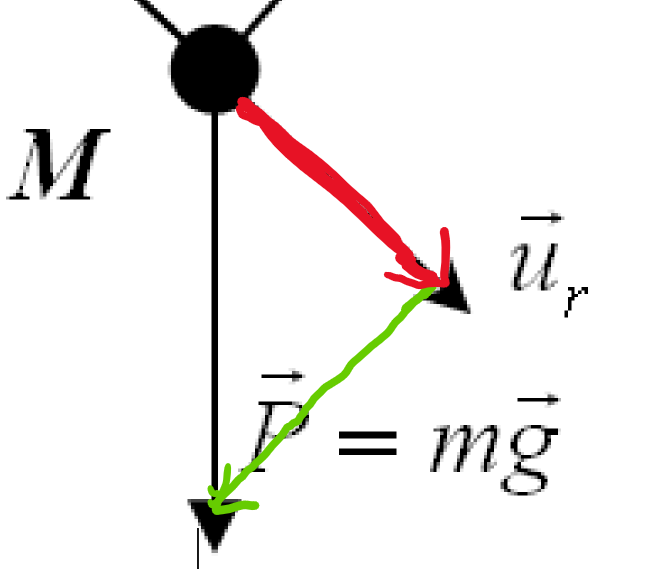
\includegraphics[scale =  0.32]{Images/Projection}

    %\end{minipage}\hfill%

    \item La projection de $\vec P$ est un peu plus ardue. Dans la base polaire, le poids peut être exprimé comme :
      \begin{equation*}
           \label{projection_poids0}
           \vec P = 
           \textrm{longueur\_flèche\_bleue}.
           \mathbf{e_r} - \textrm{longueur\_flèche\_verte}.\mathbf{e_\theta}
      \end{equation*}
      Il y a un signe '-' devant 'longueur\_flèche\_verte' car la flèche verte a un sens opposé à $\mathbf{e_\theta}$.
      Ce que l'on souhaite maintenant, c'est donc de déterminer la longueur de la flèche bleue et de la flèche verte. 
    
      
      
      %\noindent\begin{minipage}{0.2\textwidth}
    
                 %   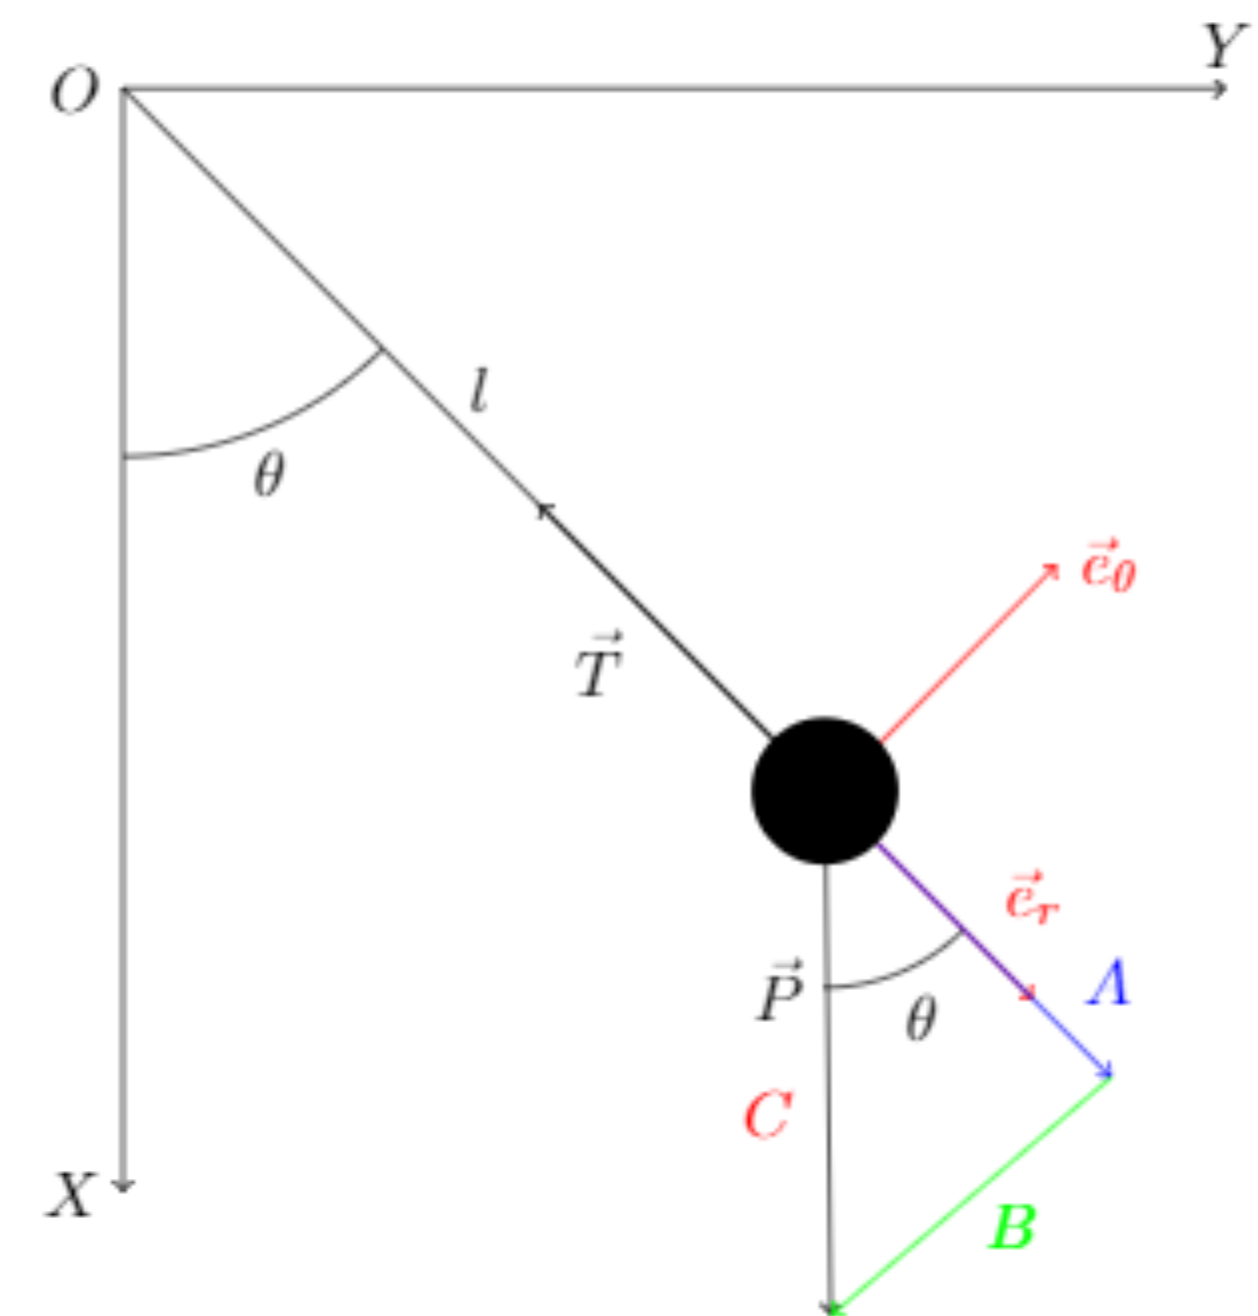
\includegraphics[scale =  0.15]{Images/Projection2}

   % \end{minipage}\hfill%
    %\begin{minipage}{\textwidth} %  
    On commence par déterminer la longueur A de la flèche bleue. Pour cela, on regarde quelles valeurs sont connues dans le triangle ABC pour pouvoir appliquer de la trigonométrie. On connaît la longueur de C, qui est $mg$. On remarque par ailleurs que l'angle entre C et A est complémentaire à l'angle $\theta$, c'est-à-dire qu'ils sont égaux. Les relations de trigonométrie donnent alors : \begin{equation*}
      \label{projection_poids1}
     \cos{\theta} = \dfrac{\textrm{Adjacent}}{\textrm {Hypoténuse}} = \dfrac{A}{C} = \dfrac{A}{mg} \iff A = mg\cos{\theta}       
     \end{equation*} 
    %\end{minipage}%
 

\noindent Maintenant que la longueur de la flèche bleue a été déterminée, on essaie de trouver celle de la flèche verte. Par les relations de trigo, on a cette fois : 
\begin{equation*}
    \label{projection_poids2}
    \sin{\theta} = \dfrac{\textrm{Opposé}}{\textrm {Hypoténuse}} = \dfrac{B}{C} = \dfrac{B}{mg} \iff B = mg\sin{\theta}    
\end{equation*}
Finalement, la décomposition de $\vec P$ dans la base polaire est donnée selon les équations précédentes par : 
\begin{equation*}
    \vec P = mg\cos{\theta}\mathbf{ e_r}-mg\sin{\theta}\mathbf{e_\theta}
\end{equation*}

\item On pose par ailleurs $a_r$ la composante radiale de l'accélération et $a_\theta$ la composante angulaire. \\
\end{itemize} 
\indent \textbf{4-} Maintenant que tous les vecteurs ont été exprimés sur la base polaire, on revient sur la deuxième loi de Newton, qui devient :
\begin{gather}
    m\vec a = \vec T + m\vec g  \iff   ma_r\mathbf{e_r} + ma_\theta\mathbf{e_\theta} = (mg\cos{\theta} - T)\mathbf{e_r}  -mg\sin{\theta}\mathbf{e_\theta}  \\
    \iff \begin{pmatrix} ma_r \\
     ma_\theta 
    \end{pmatrix} = \begin{pmatrix} mg\cos{\theta} - T \\
     -mg\sin{\theta} 
    \end{pmatrix}
    \label{equa_pendu}
\end{gather}
On se rappelle qu'en coordonnées polaires on a :
\[\begin{cases} a_{\theta} =  2\dot r\dot \theta + r\Ddot{\theta} \\
 a_{r} = \ddot r - r{\dot\theta}^2  \end{cases} \]
En insérant ces termes dans l'équation \ref{equa_pendu}, et en divisant par $m$, on a :
\begin{equation*}
\begin{pmatrix} 
      \ddot r - r{\dot\theta}^2  \\
     2\dot r\dot \theta + r\Ddot{\theta}
\end{pmatrix} = 
\begin{pmatrix} g\cos{\theta} - \dfrac{T}{m} \\
     -g\sin{\theta} 
\end{pmatrix}
\label{equa_pendu_2}
\end{equation*}
Comme la masse est contrainte à se déplacer dans un rayon $l$ autour de l'origine, on a que $r = l \implies \dot r = \ddot r = 0 $. L'équation \ref{equa_pendu_2} devient alors : 
\begin{equation*}
\begin{pmatrix} 
       -l{\dot\theta}^2  \\
       l\Ddot{\theta}
\end{pmatrix} = 
\begin{pmatrix} g\cos{\theta} - \dfrac{T}{m} \\
     -g\sin{\theta} 
\end{pmatrix}
\end{equation*}
L'égalité précédente présente deux équations du mouvement. Comme dit précédemment, le système a un seul degré de liberté étant donné qu'il suffit d'une seule coordonnée, $\theta$, pour décrire intégralement le mouvement du pendule. Nous avons donc besoin de résoudre qu'une seule des équations du mouvement.
Nous choisissons de nous attaquer à l'équation différentielle $l\ddot \theta = -g\sin{\theta} $ car elle est plus commode et ne fait pas intervenir la tension, qui est inconnue.\\

\textbf{5-} Nous ne connaissons pas encore de méthode pour résoudre l'équation différentielle $\ddot \theta = -\dfrac{g}{l}\sin{\theta}$. Il est donc nécessaire de la transformer pour la rendre plus abordable. Pour cela, on va effectuer un développement limité de la fonction $\sin{\theta}$ autour de $\theta = 0$. Il est précisé dans l'énoncé que les oscillations sont de faible amplitude, cela signifie la plupart du temps que vous devrez effectuer un développement limité.

En suivant la formule des développements limités donnée dans le cours de Mathématiques II, le développement limité de $\sin{\theta}$ à l'ordre 1 autour de 0 est donné par : 
\begin{equation*}
    \sin{\theta} \approx \sin{0} + \dfrac{\cos{0}}{1!}(\theta-0) = \theta.
\end{equation*}
En posant $\omega_0^2 = \dfrac{g}{l}$, l'équation différentielle devient 
\begin{equation*}
    \ddot \theta = -\omega_0^2\theta
\end{equation*}
Or cette équation différentielle correspond à l'équation d'un oscillateur harmonique que l'on sait résoudre !
La solution d'une telle équation est comme vu précédemment : 
\[ \theta(t) = A\cos(\omega_0 t) + B\sin(\omega_0 t) \]
\[ \dot \theta(t)= B\omega_0\cos(\omega_0 t) - A\omega_0\sin(\omega_0 t) \]
Avec $A$ et $B$ des constantes qu'on peut déterminer grâce aux conditions initiales : 
\[ \dot \theta(0) = B\omega_0  = 0 \qquad \textrm{car la vitesse initiale est nulle} \Rightarrow B = 0 \qquad \]
\[ \theta(0) = A = \theta_0 \] 
L'équation horaire du pendule est finalement donnée par : 
\[ \theta(t) = \theta_0\cos(\omega_0 t) \]

\section*{Derniers mots et remerciements} 
\noindent J'espère que cette introduction à la mécanique vous aidera au cours du semestre. Il y a encore tant de belles choses que vous découvrirez pendant le semestre, notamment le chapitre sur  \textit{l'énergie}, ou encore celui sur \textit{les moments}. Vous trouverez sur le drive les exercices qu'on vous propose, qui abordent les notions vues dans le cours.\\

\noindent Vous l'imaginez bien, de nombreuses personnes ont participé à l'élaboration de ce document. Je remercie tout d'abord les co-auteurs de ce document, Aymeric Labarbe, Gaétan Kaouadji et Joshua Freeman, qui ont passé énormement de temps à rédiger des chapitres et à corriger mes honteuses erreurs. Je tiens aussi à remercier Jonas Daverio, Louis Martins Gonçalves, Julien Ruppen, Khadija Tagemouati, Ghita Tagemouati, Youssef Amine et Gilles-Henry Moreillon, pour leur participation de près ou de loin à ce projet. J'aimerais aussi remercier tous les relecteurs Salim Najib, Yohan Abhessera, Youssef Amtine, Léo Bernard, Christelle Lam, Leila Aissa, Thibault Czarniak. Finalement j'aimerais remercier toute l'équipe de S4S en général, les speakers, les assistants, l'équipe logistique, l'équipe de communication, etc, toutes les personnes qui ont rendu ce magnifique projet possible. \\

\noindent Bonne chance et bon courage ! \\

\noindent Elias Myers \\

\noindent Pour toute suggestion ou erreur, n'hésitez pas à me contacter par mail elias.myers@epfl.ch ou par discord (eliasmyers\#7088)



\newpage

\import{Exercices/}{Exercices.tex}
\newpage
\import{Exercices/}{Corrigés.tex}
\newpage

%ERREUR, règle ça ! :angry: 
%ELias, leader ou pas, gare à toi.
%La ligne 1859 
%ah c'est pas moi :angel:
%1859 an de grâce
%mais tkt il relit tout d'abord avant d'écrire l'épilogue 
%je vais relire avec lui alors
%bien vu, je vais lire méca II

\end{document}
